\documentclass[12pt,oneside,a4paper]{report}

\usepackage{ucs}
\usepackage[utf8]{inputenc}
	\PrerenderUnicode{ěščřžýáíéĚŠČŘŽÝÁÍÉďťňĎŤŇůúÚóÓ}

\usepackage[czech]{babel}
\usepackage[IL2]{fontenc}
\usepackage[automake, nogroupskip]{glossaries}
\makeglossaries
\loadglsentries{zkratky}

\usepackage{ulem}
\usepackage{parskip}
\usepackage{pdfpages}
\usepackage{graphicx}
\usepackage{float}
\usepackage[compact]{titlesec}
%\usepackage{hyperref} % for electronic version
\usepackage[hidelinks]{hyperref} % for printing
\usepackage{svg}
\usepackage[export]{adjustbox}
\usepackage{longtable}
\usepackage{xcolor,colortbl}

\usepackage[top=2.5cm, bottom=3.5cm, left=3.5cm, right=2.5cm]{geometry}
\usepackage{graphicx}
\graphicspath{ {fig/} }
\renewcommand{\baselinestretch}{1.5}
\newcommand{\blank}[1]{\hspace*{#1}}

\DeclareCaptionType{equationcap}[][Seznam rovnic]
\captionsetup[equationcap]{name=Rovnice}
\DeclareCaptionType{graph}[][Seznam grafů]
\captionsetup[graph]{name=Graf}

\usepackage{filecontents}
\usepackage{pgfplots, pgfplotstable}

\usepackage{afterpage}
\newcommand\blankpage{
    \null
    \thispagestyle{empty}
    \newpage
}

\titleformat{\chapter}[display]
    {\normalfont\Large\bfseries}{\chaptertitlename\ \thechapter\Makeuppercase}{20pt}{\Large}
\titlespacing*{\chapter}{0pt}{0pt}{10pt}

\titleformat*{\section}{\large\bfseries}
\titleformat*{\subsection}{\normalsize\bfseries}

\makeatletter
\renewcommand{\@makechapterhead}[1]{
{\setlength{\parindent}{0pt} \raggedright \normalfont
\bfseries\Large\thechapter\ #1
\par\nobreak\vspace{10 pt}}}
\makeatother
\setlength{\parindent}{2em}
\setlength{\parskip}{0cm}
%------------------------------------------------------------------------------------------------------------------------------------------
%  Začátek dokumentu
%------------------------------------------------------------------------------------------------------------------------------------------
\begin{document}

%------------------------------------------------------------------------------------------------------------------------------------------
%  Titulní list
%------------------------------------------------------------------------------------------------------------------------------------------
\pagestyle{empty}

\includepdf[pages={1}]{TitulniList_color.pdf}
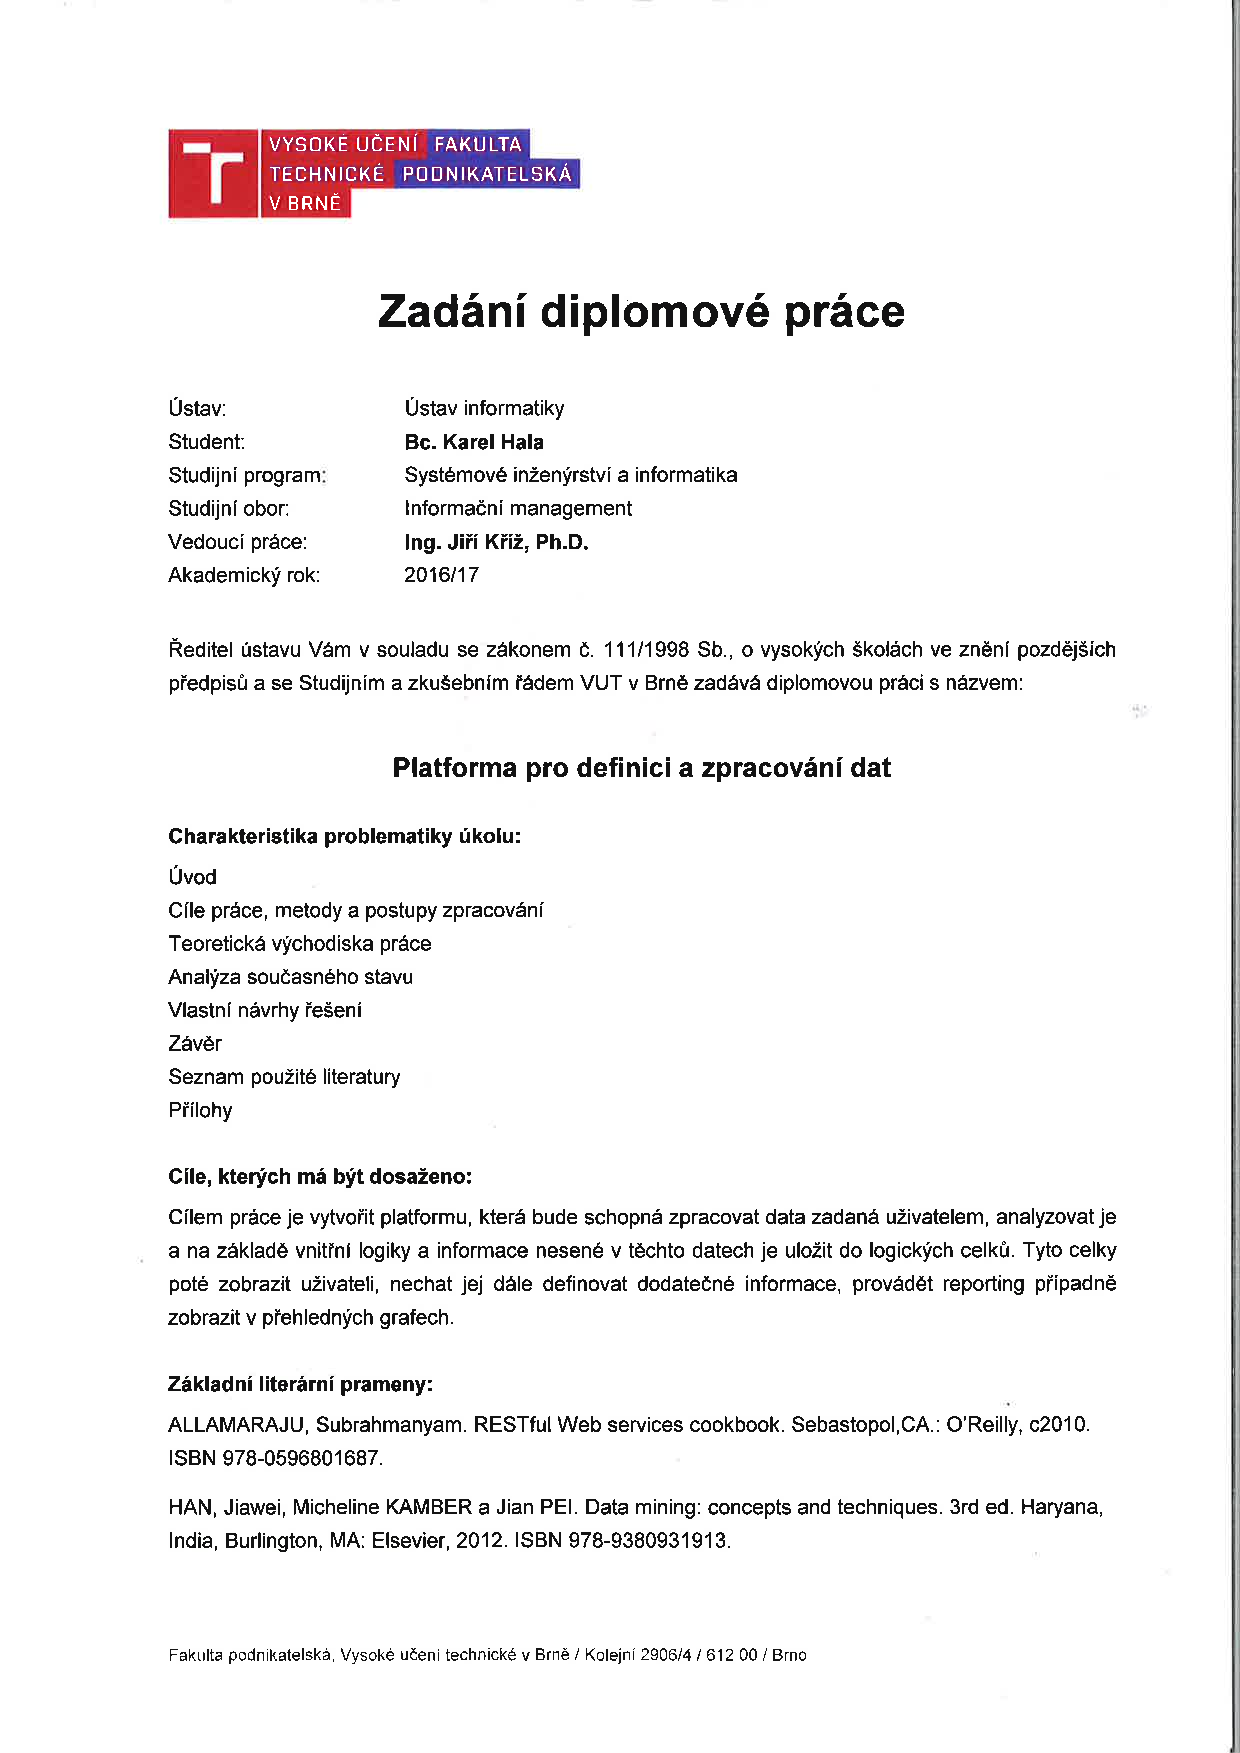
\includepdf[pages={1,2}]{zadani_podepsane.pdf}

%------------------------------------------------------------------------------------------------------------------------------------------
%  Abstrakt
%------------------------------------------------------------------------------------------------------------------------------------------
\section*{Abstrakt}
Tato diplomová práce se zabývá vývojem platformy pro ulehčení práce s~velkým množstvím dat. V~rámci této práce jsou vysvětleny některé pojmy a technické souvislosti potřebné pro bližší pochopení vývoje webové aplikace. Dále jsou zde navrženy postupy, jak usnadnit uživateli zadávání a práci s~větším objemem dat. Platforma je koncipována tak, aby bylo možné jednoduše a rychle rozšířit jakoukoliv část.
\section*{Summary}
This diploma thesis deals with creating platform which serves for easy manipulation with large data set. There are numerous technical knowledge described in this thesis to understand web development. Later there are proposed approaches of how to make as easy as possible for user to define and work with large data sets. Platform is written and created in a way, that it is easy to extend eny part of it.

\hbox{}
\vfill

%------------------------------------------------------------------------------------------------------------------------------------------
%  Klíčová slova
%------------------------------------------------------------------------------------------------------------------------------------------
\section*{Klíčová slova}
big data, podpůrný nástroj, webová aplikace, uživatelské rozhraní
\section*{Key words}
big data, supportive tool, web application, user interface
\vskip1cm

\newpage
\hbox{}
\vfill

%------------------------------------------------------------------------------------------------------------------------------------------
%  Bibliografická citace
%------------------------------------------------------------------------------------------------------------------------------------------
\section*{Bibliografická citace}
HALA, K. \textit{Platforma pro definici a zpracování dat}. Brno: Vysoké učení technické v~Brně, Fakulta podnikatelská, 2017. 82 s. Vedoucí diplomové práce Ing. Jiří Kříž, Ph.D..
\vskip1cm

\newpage
\hbox{}
\vfill

%------------------------------------------------------------------------------------------------------------------------------------------
%  Prohlášení
%------------------------------------------------------------------------------------------------------------------------------------------
\section*{Čestné prohlášení}
Prohlašuji, že předložená diplomová práce je původní a zpracoval jsem ji samostatně. Prohlašuji, že citace použitých pramenů jsou úplné a že jsem ve své práci neporušil autorská práva (ve smyslu Zákona č. 121/2000 Sb., o~právu autorském a~o~právech souvisejících s~právem autorským).
\\
\par V~Brně dne 24. 5. 2017 % doplnit datum
\hfill\dotuline{\blank{5cm}}\hskip2cm
\par\hfill jméno \hskip5cm\blank{-4cm}
\vskip1cm

\newpage
\hbox{}
\vfill

%------------------------------------------------------------------------------------------------------------------------------------------
%  Poděkování
%------------------------------------------------------------------------------------------------------------------------------------------
\section*{Poděkování}
Rád bych poděkoval panu Ing. Jiřímu Křížovi, Ph.D. za vedení a konzultace během této práce. Dále bych chtěl poděkovat rodině a partnerce za morální podporu.
\vskip1cm

%------------------------------------------------------------------------------------------------------------------------------------------
%  Obsah
%-----------------------------------------------------------------------------------------------------------------------------------------
\renewcommand{\baselinestretch}{1}
\tableofcontents

\addtocontents{toc}{\protect\thispagestyle{empty}}

%------------------------------------------------------------------------------------------------------------------------------------------
%  Vlastní texty
%------------------------------------------------------------------------------------------------------------------------------------------
\renewcommand{\baselinestretch}{1.5}

%------------------------------------------------------------------------------------------------------------------------------------------
% Úvod
%------------------------------------------------------------------------------------------------------------------------------------------
\chapter*{ÚVOD}
\addcontentsline{toc}{chapter}{ÚVOD} 
\par V~aktuální době je velké množství dokumentů ve firmách zpracováváno nástroji, které do jisté míry nepodporují spolupráci a často tak dochází k~vytváření velkých a nepřehledných dokumentů, které se časem zvětšují a po několika letech se musí kompletně přepsat a případně zrušit.

\par S~nástupem internetu tento problém částečně vymizel díky tomu, že se nyní dají takové dokumenty velice snadno sdílet, nicméně stále je zde problém, že velká část nástrojů pracujících s~dokumenty nenabízí jednoduché a přehledné provázání. Proto se v~rámci této práce zaměříme na možná řešení některých problémů, které vznikají při sdílení dokumentů a při jejich propojování.

\par Cílem této práce je tedy analýza současných nástrojů a následně návrh a vytvoření specifického nástroje, který se bude zaměřovat z~velké části na jeho snadné používání uživateli.

\par Diplomová práce nás postupně provede několika kapitolami, kdy se nejdříve budeme věnovat teoretickým východiskům, kde si vysvětlíme některé pojmy zabývající se prací s~dokumenty pomocí webových aplikací, poté se zaměříme na aktuální stav nástrojů a aplikací zabývajících se touto problematikou. Část popisu aktuálního stavu se budeme věnovat nástrojům, které nám mohou pomoci při samotném vývoji aplikace. Na samotný návrh a vývoj aplikace se zaměříme v~poslední kapitole, ve které si rozebereme také případná rizika vývoje takového nástroje. Od čtenáře se očekávají alespoň základní technické znalosti vývoje aplikací a prací s~webovými technologiemi.

%------------------------------------------------------------------------------------------------------------------------------------------
% Cíl a metodika práce
%------------------------------------------------------------------------------------------------------------------------------------------
\chapter*{CÍL DIPLOMOVÉ PRÁCE}
Hlavním cílem této práce je vytvořit platformu, která bude schopná zpracovat data zadaná uživatelem, analyzovat je a na základě vnitřní logiky a informace nesené v~těchto datech je uložit do logických celků. Aplikace poté umožní tyto celky zobrazit uživateli, nechá jej dále definovat dodatečné informace, provádět reporting a případně zobrazit v~přehledných grafech.

Platforma se bude zaměřovat převážně na uživatelské rozhraní, tak aby její používání bylo co nejintuitivnější a nejjednodušší.
\addcontentsline{toc}{chapter}{CÍL DIPLOMOVÉ PRÁCE}

\chapter*{METODIKA PRÁCE}
\addcontentsline{toc}{chapter}{METODIKA PRÁCE}
\section*{Metody}
\par Nejdůležitějším zaměřením této platformy je uživatelská přívětivost a jednoduchost na používání, proto bude při vývoji kladen důraz na spokojenost uživatelů. Tohoto bude dosaženo použitím agilních metodik při vývoji, kdy bude postupně dodávaný produkt předáván úzkému kruhu uživatelů, kteří se budou vyjadřovat k~uživatelskému rozhraní. Platforma bude psána jako webová aplikace, která bude přistupovat do databáze přes rozhraní napsané v~jazyce Java.
\par V~části zpracování dat bude použito několik ETL metodik a data mining technik, které povedou ke získání logických informací ze zadaných dat. Platforma bude vyvíjena s~možností 
škálovatelnosti a použití nad velkým objemem dat.
\addcontentsline{toc}{section}{Metody}

\section*{Postupy}
\addcontentsline{toc}{section}{Postupy}
\par K~vytvoření co nejpřívětivější platformy budou využity naše zkušenosti a knižní publikace zabývající se tímto tématem. Dále budou analyzovány jednotlivé postupy zadávání dat uživatelů do tohoto systému, které povedou ke zpřehlednění a zjednodušení používání.
\par Pro komunikaci se serverem bude použit standard REST, který usnadní komunikaci se serverem a umožní případné navázání nových aplikací. V~případě, že bude vytvořena mobilní aplikace pro získávání dat, nebude nutné psát znovu stejnou nebo podobnou logiku.
\par Pro zabezpečené přihlášení do aplikace bude použit autentizační server, který bude zajišťovat vytváření a správu uživatelů spolu s~jejich právy.



\pagestyle{plain}     % zapne obyčejné číslování

%------------------------------------------------------------------------------------------------------------------------------------------
%  Teorie
%------------------------------------------------------------------------------------------------------------------------------------------
\chapter{TEORETICKÁ VÝCHODISKA}
\par Pro plné pochopení, výběru a případném vypracování platformz je potřeba si objasnit a vysvětlit několik témat. Jsou to především \textit{Vývojové platformy low-code}, výsledná platforma by měla splňovat tuto definici. Dále si objasníme pojemy \textit{Bussiness intelligence} (platforma bude z části pracovat s touto oblastí) a \textit{Platforma pro pokročilou vizualizaci dat} -- pro snadné používání uživatelského rozhraní. A vzhledem k tomu že výsledná platforma musí do určité části pracovat s uživatelskými právy a spravovat uživatele, objasníme si pojem \textit{Server pro řízení přístupu a identity}

\section{Vývojové platformy low-code}
\par Vývojové platformy low-code jsou celkem nový pojem, tyto produkty začali vznikat, protože malé a střední podniky potřebovali vytvořit rychle a za použití menšího počtu vývojářů aplikace, které mohou být nadále rychle spravovány. \ref{pcmag-no-coding}

\par Toto v podstatě znamená, že vývojáři mohou rychle měnit software na základě uživatelských požadavků, což má za následek spokojenější uživatele, uživatelsky přívětivější software a toto všechno za minimálního použití ručního programování. Takovéto platformy neeliminují programování jako takové, ale napomáhají rychlejšímu vývoji, tak že poskytují vizuální nástroje a napomáhají konfiguraci datových modulů a pomáhají eliminovat problémy spojené s  datovou integrací. - http://www.cio.com/article/2845378/development-tools/use-low-code-platforms-to-develop-the-apps-customers-want.html

\paragraph{Výhody low-code platforem}
\begin{itemize}
  \item \textbf{Produktivita:} Systémy mohou být vyvýjeny a nasazeny během menšího časového rozmezí, oproti klasickému programování.
  \item \textbf{Reakční schopnost:} Vývojář může často zvolit různé druhy platforem na kterých bude výsledný produkt fungvat, od mobilních aplikací, až po webové služby.
  \item \textbf{Spolehlivost:} Aplikace mohou být aktualizovány mnohem rychleji, což má za následek jejich stabilitu a spolehlivost.
  \item \textbf{Úspora času a peněz:} Vývojáři mohou vytvořit mnohem více funkcionality za kratší čas, z čehož plyne že si firma může dovolit mensí počet programátorů.
  \item \textbf{Zaměření na samotný vývoj:} Zaměřením na to co má aplikace dělat, a ne jak to má dělat, programátoři se mohou zaměřit na funkcionalitu a uživatelskou spokojenost. Při vývoji je možné se zaměřit také více na uživatelské požadavky mnohem rychleji.
\end{itemize}
http://sdtimes.com/low-code-development-seeks-accelerate-software-delivery/

\subsection{Příklady low-code platforem}
\paragraph{Microsoft PowerApps} Vývojová platforma od firmy Microsoft, která dovoluje vytvořit během několika málo kliknutí aplikaci pro mobilní platformy a také jako webové služby. Při spojením této platformy a aplikace Power BI vzniká velice robustní vývojářský nástroj, díky kterému je možné rychle integrovat produkční data do aplikace, kterou budou uživatelé rádi používat.
\paragraph{Zoho Creator} Výhodou této platformy je využití techniky \uv{\tt{drag-and-drop}}, která umožňuje vytvářet aplikace a převážně jejich uživatelské rozhraní bez nutnosti psát jakýkoliv kód. https://reviews.financesonline.com/p/zoho-creator/
\paragraph{Rollbase} Při používání této platformy vývojář jako první definuje objekty, jejich vlastnosti a vztahy mezi těmito objekty. Po překonání tohoto kroku máme již plně funkční webovou aplikaci, která je funkční napříč všemi mobilními zařízeními. https://www.progress.com/blogs/what-is-a-low-code-platform
\paragraph{Openshift} Platforma pro vývoj webovým a mobilních aplikací, postavená na kontejnerech, které zajišťuí rychlý vývoj a možnost dedikovat vývojáře na vytvoření jednoduchých funcionalit jako samostatné aplikace \footnote{Takovýmto aplikacím se říka Microservice https://smartbear.com/learn/api-design/what-are-microservices/}, které za pomocí Openshiftu vytvoří velkou a komplexní aplikaci.
\begin{figure}[h]
\centering
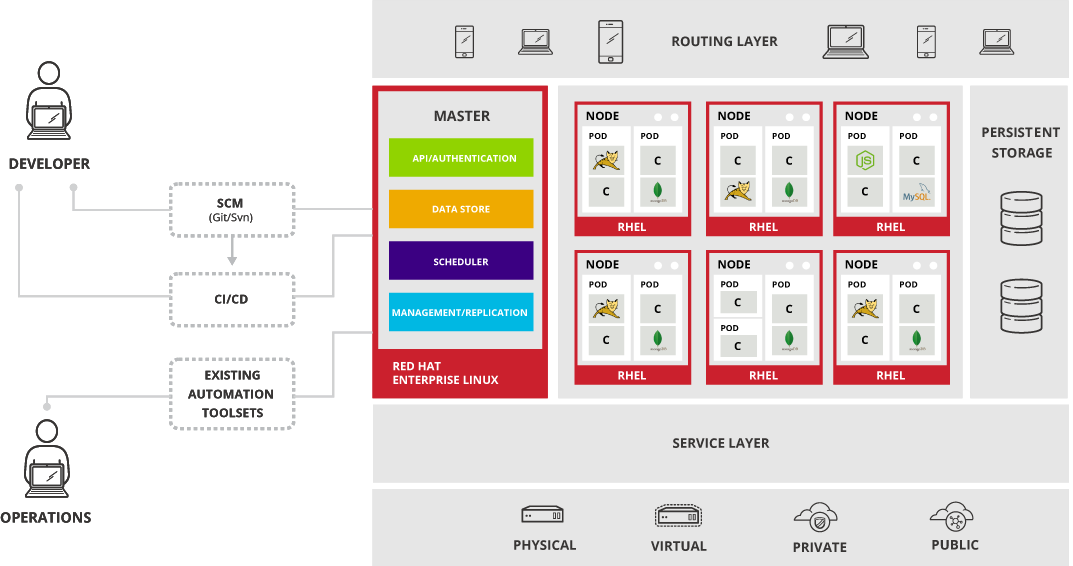
\includegraphics[width=\textwidth]{openshift}
\caption{Znozornění jednotlivých vrstev v platformě openshift.}
\end{figure}

\subsection{Platforma jako služba -- Paas}

\section{Bussiness Intelligence}

\subsection{Big data}

\subsection{Datamining}

\subsection{Extraction, Transaction, Loading}

\subsection{NoSql databáze}
\cite{nosql}

\section{Platforma pro pokročilou vizualizaci dat}
\subsection{Single page aplikace}
\subsection{Dynamická a interaktivní vizualizace dat}
\subsection{Webová služba RESTful}
Restufl web APIs

\section{Server pro řízení přístupu a identity}
\url{http://www.sersc.org/journals/IJMUE/vol9_no9_2014/9.pdf}

\subsection{JSON Web Token}
https://tools.ietf.org/html/rfc7519
https://scotch.io/tutorials/the-anatomy-of-a-json-web-token

%------------------------------------------------------------------------------------------------------------------------------------------
%  Analyza prostredku
%------------------------------------------------------------------------------------------------------------------------------------------
\chapter{ANALYTICKÁ ČÁST} \label{analyza}
\par Před samotným vývojem platformy pro definici a zpracování dat musíme provést průzkum aktuálních technologií zaměřujících se na vývoj webových aplikací a jejich výběr. Výběr echnologií, které nám pomohou při vývoji je velice podstatný, protože nám urychlí dodání a co je dležitější, pozdější úprava bude značně jednodušší pokud zvolíme technologie, které nám takovýto pozdější vývoj usnadní.

\par Nejenom vývojovími technologiemi je potřeba se zabývat, ale také aktuálním stavem trhu a toho co uživatelé nejčasteji používají. Proto se v této části zaměříme také průzkumem trhu.

\section{Webové technologie}
\par Aktuální trend v používání webových prohlížečů můžeme vidět na grafu \ref{browser-share}, kde jde jasně vidět že moderní prohlížeče v podání Chrome a Firefox převládají nad tolika vývojáří proklínaný a čím dál tím méně používaný Internet Explorer. dále si uživatelé již uvědomují, že aktualizace prohlížeče je pro zachování zabezpečení nutností a tak naštěstí webové prohlížeče pomalu začínají pořádně fungovat s novým standardem JavaScriptu nazvaný EcmaSript 6 (znáý též pod názvem ES2015 a ES6). \cite{es6}

\par Nový standard ES6 přináší mnoho vylepšení a mnoho optimalizací. Nicméně ani většina moderních prohlížečů nepodporuje 100 \% tento standard, například prohlížeč \textbf{Google chrome} ve verzi 57 podporuje 97 \% nového standardu, obdobně je na tom \textbf{Edge} (verze 15 podporuje 95 \%) a \textbf{Firefox} (verze 52 zvládá 94\%). \cite{es6-coverage}

\subsection{Webový aplikační rámec}
\par V aktuální době se mnoha vývojářům webových aplikací ověřili takzvané webové aplikační rámce. Dříve hojně využíváná knihovna  \textbf{jQuery} má již mnoho nástupců jak v podobě knihoven, tak aplikačních rámců. Výhoda takových aplikačních rámců je že se stará v podstatě o veškerou těžkou a neustále se opakující práci a nechává programátorovi volnou ruku při realizaci samostatné aplikace. \cite{framework}

\par V předešlém odstavci bylo použito obou pojmů, jak JavaScriptové knihovny, tak aplikačního webového rámce. Tyto pojmy dost často vedou k hádkám a nedorozumění, kdy valná většina programátorů nerozumí rozdílům mezi aplikačním rámcem a knihovnou.
\begin{itemize}
  \item \textbf{JavaScriptová knihovna} slouží ke konání jednoho úkolu. Vezměme si například výrobu kávy, můžeme si postavit vodu na oheň ohřát ji, rozemlít zrnka kávy a tento prášek zalít horkou vodou. Každý jeden nástroj by představoval knihovnu.
  \item \textbf{Aplikační webový rámec} má na starosti veškerou práci a často zahrnuje přesně definovanou architekturu. Pokud si vezmeme příklad s kávou, aplikační webový rámec by byl kávovar, do kterého nalijeme vodu a nasypeme kávová zrna. \cite{framework-vs-library}
\end{itemize}

\paragraph{Angular.js} je plnohodnotný aplikační rámec, v aktuální době pravděpodobně nejpoužívanější. \footnote{Přesná čísla se určit nedají, nicméně více informací o popularitě se můžete dočist zde: \url{https://hackernoon.com/5-best-javascript-frameworks-in-2017-7a63b3870282\#.ufk9gznfd}}.

\par Strukturální webový aplikační rámec, pro dynamické webové aplikace. Jeho přední výhodou je že se soustřeďuje na tvoření jednostránkových aplikací. Takže často snižuje počet dat nutných pro načtení apracování s aplikací. První datum vydaní bylo v roce 2010 a v roce 2016 byla vydána verze 2, která umožňuje vytvářet uživatelské rozhraní jak pro webové, tak pro mobilní aplikace.\cite{angular-js}

\paragraph{React.js} není plnohodnotný aplikační rámec, jako \textbf{Angular.js}, nicméně je velkým hráčem na poli vývoje webových aplikací. Jeho výhodou je jeho jednoduchost, nastavení aplikace a počáteční vývoj je velice jednoduchý, nicméně nedokáže tolik věcí co plnohodnotný rámec. Samostatný ovšem není příliš vhodný, potřebuje několik rozšíření, které z něho udělají silnějšího hráče, to ale vede k jeho yesložitění a častým problémům s nastavením. \cite{react-js}

\paragraph{Vue.js} je progresivní rámec, pro vytváření uživatelských rozhraní. Jeho tvůrci kladli důraz na jeho jednoduchost použití a inspirovali se v \textbf{React.js}, výhodou oproti zmíněnému má použití s webovou stránkou, kdy se nesnaží obcházet její vykreslování, ale pracuje přímo s html elementy. Dále je tento rámec také zaměřen na práci s jednostránkovou aplikací, takže je výborným kompromisem mezi \textbf{Angular.js} -- který může být příliš náročný pro pochopení, a \textbf{React.js} -- který může vést k zesložitění při použití s více rozšířeními. \cite{vue-js}

\subsection{Silné vs. slabé typování}
\par Pro vývoj responzivních webových aplikací se používá JavaScript, který je ale slabě typovaný. To znamená že proměnná nemá předem určený pevný typ a může ho během chodu aplikace měnit. To může mít za následek chyby spojené s očekávaným typem, který může být chybný. Takže například při očekávání čísla budeme sčítat, ale aplikace nám během jejího chodu vrátila text. Takový problém může vést až k pádu, případně zamrznutí aplikace. Proto vznikl způsob jak přivést silné typování do slabě typovaných jazyků, jejich zástupci jsou \textbf{Typescript} a \textbf{Flow}.

\paragraph{Typescript} je podmnožinou JavaScriptu, to znamená že veškeré soubory jsou přeloženy do předem vybrané verze specifikace a ty jsou poté spuštěny v prohlížeči. Není tedy nutné nutit uživatele do používání jiného prohlížeče. Velkou výhodou je také to, že se tým okolo Typescriptu snaží co nejvíce sledovat trend vývoje JavaScriptu a tak přináší mnoho novinek ještě před tím, než je začnou používat prohlížeče. Takže je možné použít velkou část nových technologií, bez nutnosti psát ne zrovna příjemně čitelný kód. \cite{typescript}

\paragraph{Flow} je další způsob jak přivést silné typování do světa JavaScriptu, oproti \textbf{Typescriptu} má výhody, že problémy s implicitní deklarací, které mohou nastat během používání aplikace jsou lépe vyhodnoceny a programátor je o tomto informován již během překladu aplikace. Ale jeho nevýhodou je, že nesleduje takovou měrou nejnovější trendy a je často pozadu. Někdy schválně, protože pro překlad novějších definic do staršího použití existují další nástroje. \cite{flow}

\subsection{Responzivní aplikační rámec}
\par Pro usnadnění používání webových aplikací na jekémkoliv zařízení vzniká aktuálně mnoho knihoven a aplikačních rámců, které mají za úkol sjednotit design napříč několika aplikacemi a také jejich responzibilitu. To znamená že stejná aplikace se bude chovat a vypadat stejně bez ohledu na to, na jakém zařízení ji otevřeme (mobilní zařízení, tablet, počítač, televize, atd.)

\paragraph{Material design} vznikl na popud zjednodušení a zpřehlednění uživatelského rozhraní, jeho hlavním zaměřením je dotek, hlas a kliknutí. Definuje tři pravidla \textbf{Material je metafora} -- chytře využívat prostor a pohyb jednotlivých elementů. \textbf{Tučné, grafické, záměrné} -- základními stavebními bloky jsou typografie, mřížka, místo, barva a použití obrázků. \textbf{Pohyb má význam} -- pokud uživatel vykoná nějakou akci design mu napoví jaká akce se stane pohybem. \cite{material}

\paragraph{Boostrap} jeden z prvních responzivních rámců, který přivedl sjednocení uživatelského rozhraní napříč všemi platformami s největším důrazem na mobilní platformy. Dost často jsou vytvořeny webové aplikace, které nerespektují různé rozlyšení pro různé uživatele, tomuto se chtěl bootstrap vyhnout. Nyní nabízí velké množství doplňků a rozšíření, díky kterým z něj dělají rávem nejrozšířenější responzivní rámec. \cite{bootstrap}

\paragraph{Patternfly} se inspiroval bootsrapem a vytvořil vlastní responzivní rámec, dále nabízí několik widgetů pro zobrazování složitějších uživatelských dat. Jeho hlavním zaměřením je unifikovat jednotlivé aplikace ve firmě, tak aby měli stejný, ale unikátní design. Proto nabízí několik jednoduchých přístupů co a jak dělat pro dosažení co nejvíce podobného vzhledu napříč aplikacemi. \cite{patternfly}

\section{Single sign-on}
\par V aktuální době velká část společností nabízejících větší potrfolio aplikací volí takzvanou službu single sign-on, kdy uživatel nemusí pokaždé zadávat své přihlašovací údaje, ale o jeho identifikaci se postará specializovaná služba. Většinou se stačí do této služby přihlásit jednou a dokud nevyprší čas od posledního použití aplikace, která používá tuto službu, nebo není uživatel schválně  odhlášen nemusí se znovu přihlašovat. Jako protiklad je postaven Single sign-off, kdy při odhlášení v jedné aplikaci je uživatel automaticky odhlášen ze všech ostatních aplikací, toto napomáhá dalšímu zabezpečení.

\subsection{Standardy získání identity}
\par V aktuální době jsou pravděpodobně nejrozšířenější dva standardy použití SSO -- novější \textbf{OpenID Connect} a starší, ale robustnější \textbf{SAML}.
\paragraph{OpenID Connect} je v podstatě identitní vrstva postavená nad OAuth 2.0, poskytuje možnost identifikace uživatele a také získání základních informací. Modernější a v aktuální době více používaný způsob převážně kvůli jeho jednoduchosti a nižšímu zatížení serveru. \cite{oidc}

\paragraph{SAML} se skládá ze dvou částí, poskytovatele služby a poskytovatele totožnosti (tím může být například Facebook, Google, Github, atd.). Jakým způsobem je uživatel přihlášen do služby můžeme vidět na obrázku \ref{saml2}. Nejdříve uživatel vytvoří požadavek na poskytovatele služby, ten vygeneruje SAML požadavek v URL, aplikace přesměruje uživatele na poskytovatele totožnosti, ten ověří přihlašovací údaje, přepošle zpět na poskytovatele služby požadavek na potvrzení, dále je uživatel přesměrován na cílový požadavake, o který si znovu požádá a server mu jej vrátí. \cite{saml}
\begin{figure}[hp]
  \centering
  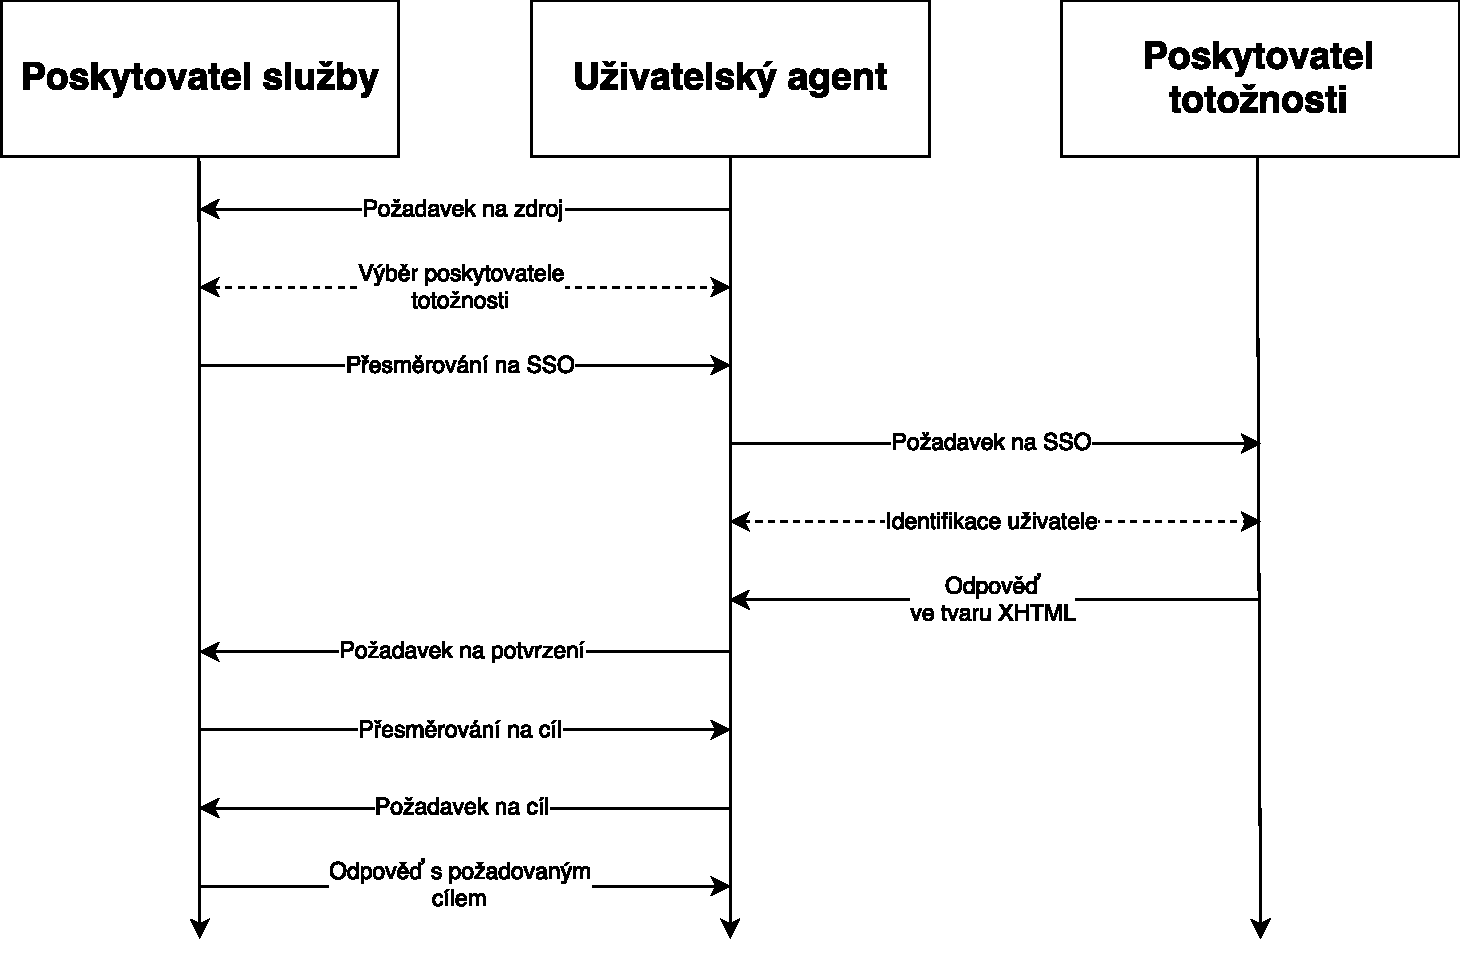
\includegraphics[max size={\textwidth}{\textheight}]{SAML2.pdf}
  \caption{Předání uživatelského požadavku při použití SAML2}
  \label{saml2}
\end{figure}

\subsection{Autentikační servery} \label{auth-server}
\par Aktuální trh nabízí velké množství autentikačních serverů, které spravují uživatele a poskytují přihlášení do více aplikací. Některé jsou dokonce volně k použití bez nutnosti zakoupit licenci, je nutné pouze spravovat servery na kterých takováto služba poběží.

\paragraph{Keycloak} je open sourcové řešení, které nabízí připojení jak přes sociální síťe a možnost získání uživatelských účtů z LDAP, Active Directory a nebo přímo z databáze. Jeho velkou premisou je jednoduchost správy uživatelů, včetně definice přístupových práv pro jednotlivé části aplikace. \cite{keycloak}
\paragraph{Sterling externí autentikační server} je řešení od IBM nabízející rozšířené autentizace a validace služeb pro IBM produkty, nabízí napojení například na LDAP a možnost SSH autentizace. \cite{ibm-ster}
\paragraph{Active Directory Federation Services} od firmy Microsoft nabízí možnost sdílet identifikační informace napříč důveryhodným obchodním partnerům skrze extranet. Výhodou je že se nemusí aplikace starat o všechny uživatele, ale pouze si vyžádá od spřátelené aplikace jeho práva.  \cite{ADFS}

\section{Datová analýza}
\par Pokud firma disponuje velkým množstvím dat je vhodné nad těmito daty najít nějaké souvislosti, které jí dopomůžou k vytváření dalšího zisku, případně pouze pro pochopení daného zákazníka, nebo skupiny zákazníků. Pokud je těchto dat opravdu hodně, můžeme je označit za Big Data (popsáno v \ref{big-data}), poté procesům k získání dalších informací říkáme Dolování dat (blíže popsáno v \ref{data-mining}).

\subsection{Shluková analýza}
\par Pro bližší pochopení velkého množství dat je vhodné použít metodu shlukoví analýzy, což je zjednodušené proces organizace objektů do skupin, tak aby její člonové byli nějakým způsobem co nejvíce podobní. Shlukovou analýzu můžeme rozdělit do dvou skupin \textbf{nehierarchické} a \textbf{hierarchické}.

\paragraph{Nehierarchické} metody mohou být tvrdé nebo jemné, tvrdé seskupují data na základě specifické shlukové vlastnosti -- pokud patří do tohoto shluku namůže patřit do jiného. Jemné na druhou stranu nedefinují přesnou hranici -- patří do tohoto shluku, ale má některé vlatnosti daotových bodů jiných shluků. Pro dělení můžeme použít metodu K-means, která přiřadí každý bod do shluku jemuž středu je nejblíže a při každém běhu algoritmu se středy shluků přepočítávají jako aritmetické průměry všech bodů.

\paragraph{Hierarchické} metody můžeme použít ve dvou způsobech ze shora dolů a odspodu nahoru. V prnvím případě vezmeme všechny datové body a označíme jej za shluk, který poté rozdělíme na další shluky, které dále dělíme. Opět můžeme využít K-means pro dělení shluků. Druhý způsob (odspodu nahoru) je nejlépe použít v případě že máme menší vzorek dat a chceme co nejlepší shluk.

\par Pro shrnutí je potřeba si uvědomit dvě věci, jaký je nejmenší počet shluků a naopak jaký je největzší počet těchto shluků. Na první otázku je jednoduché odpovědět, je to v podstatě celý seznam datových bodů v jednom shluku (není nám to příliš užitečné, ale je to shluk dat). Na otázku největšího počtu shluků můžeme říct, že jím je počet všech datových bodů (toto opět není příliš užitečné). Proces shlukování je tedy rozdělování těchto dat do shluků větších jak jedna a menších než počet prvků, proces ukončíme v momenté, kdy jsme spokojeni s celkovým počtem shluků, případně velikostí těchto skupin.

\subsection{Rozhodovací stromy}
\par Tento algoritmus slouží k získání pravidel a vztahů v datovém souboru pomocí větvení. Díky použití stromů je tento algoritmus rychlý a výhodný pro použití s počítačem. Složení stromu je takové že na vrcholu je jeden uzel, kterému se říká kořen, ze kterého vede několik hran spojující vnitřní uzly, které mají opět několik hran projujících další uzly. Každý uzel musí mít právě jednoho předka (ne více ani méně), kromě kořenového uzlu, který nemá žádného předka. Výhodou je jednoduchost, efektivnost a možnost použít i pro velký objem dat, na druhou stranu pokud nám budou některá data chybět, nebo budeme mít spojitá data rozhodovací stromy budou mít problémy. Při výběru vlastnosti, která je nejvíce odlišná od ostatních příkladů v ostatních třídách se požívá takzvané entropie, její výpočet lze vidět na \ref{entropie}, kde \(p_t\) je pravděpodobnost výskytu třídy \(t\) a \(t\) je počet tříd
\begin{equation} \label{entropie}
E(S) = - \sum_{t=1}^{T}(p_t log_2 p_t)
\end{equation}

\par Pro vytvoření stromu se vezme tabulka hodnot a pro každý atribut se vypočítá jeho entropie, ta znázorňuje homogenitu prvku. Pokud je prvek naprosto homogenní (nácházející se ve všech atributech) jeho entropie je 0, naopak pokud je prvek naprosto heterogenní (nachází se pouze v jednom atributu) jeho entropie je 1. Při prvnotním vytvoření rozhodovacího stromu je tedy potřeba mít co nejlepší trénovací data, nicméně velké množství dat může mít za následek příliš složitý strom, který je opět nepoužitelný (proto je potřeba dbát na vhodnou velikost učebních dat). Pokud nám vznikne složitý a ne příliš efektivní rozhodovací strom je vhodné použít takzvané prořezávání, kdy odstraníme nadbytečné podstromy (velice vhodné v případě že jsme použili velký vzorek dat pro vytvoření stromu).

\par Příklad algoritmu, který se používá pro vytváření rozhodovacích stromů je takzvaný ID3, je založen na booleanovských hodnotách, používá hladové vyhledávání v prostoru \footnote{Pro bližší informace o hladovém prohledávání \url{http://www.how2examples.com/artificial-intelligence/tree-search}} a strom je vytvářen odshora dolů. Vstupní parametry tohoto algoritmu jsou \textbf{příklady} -- data na kterých je rozhodovací strom vytrénován \textbf{atributy} -- nad nimiž ude strom testován a \textbf{cílový atribut} -- tento atribut se bude vytvořený strom snažit predikovat. ID3 algoritmus byl několikrát vylepšen a upraven pro použití za různých podmínek jako například C4.5 (vhodné při chybejících, nebo spojitých datech), C5 (vylepšený C4.5), pro vytvoření binárních rozhodovacích stromů je například vhodné použít klasifikační a regresní stromy (CART), případně pro práci s opravdu velkým množstvím dat je možné použít algoritmus SPRINT.

\par Na obrázku \ref{decision-tree} můžeme vidět příklad stromu, který vznikl pro rozhodování zda jít hrát badminton, pro jeho vytvoření byl použit algoritmus ID3 s menším vzorekem dat.
\begin{figure}[htp]
  \centering
  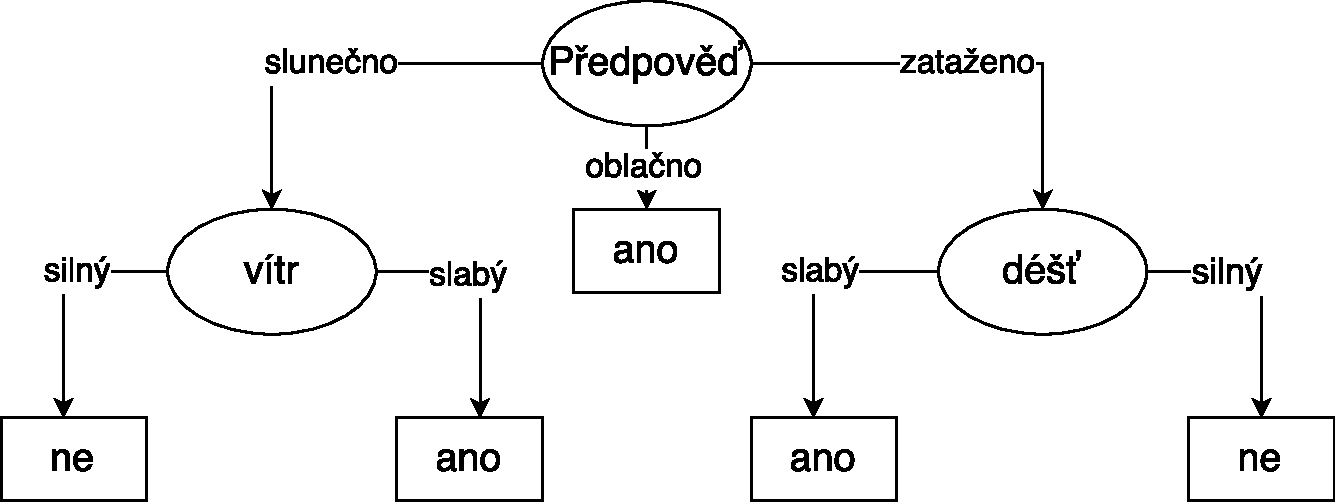
\includegraphics[max size={\textwidth}]{decision.pdf}
  \caption{Příklad rozhodovacího stromu při použití algoritmu ID3.}
  \label{decision-tree}
\end{figure}


\subsection{Dolování dat na webové aplikaci}
\par Toto získávání dalších informací z dat je v podstatě dolování z webových dokumentů, hyperlinků mezi nimi a získání informací z logů a webových stránek. \cite{minigbook}

\par Na webu lze využít několik možných technik dolování:
\begin{itemize}
  \item \textbf{Webového obsahu} je proces získávání informací z webových dokumentů, mohou to být jak samotné stránky, tak videa, zvukových stop a obrázků. Hlavním zaměřením je však získání informací ze samotných textů na webovém dokumentu.
  \item \textbf{Webové struktury} strukturu webových stránek si lze představit jako, uzlový graf, ve kterém jednotlivé uzly jsou samotné stránky a hrany spojující tyto stránky jsou vzájemné odkazy. Lze se také dále zanořit v jednotlivých dokumentech a ty znázornit pomocí stromové struktyry \footnote{Přesný popis tohoto zápisu je znám pod zkratkou DOM (Document object model) \url{https://www.w3.org/TR/DOM-Level-2-Core/introduction.html}}.
  \item \textbf{Webového použití} je název pro označení technik, díky kterým lze získat další informace z používání webových stránek. Tyto data lze získat z několika zdrojů \textbf{webový server} -- záznamy, které vygeneroval server během jeho používání (IP adresy uživatelů, navštívenou stránku a čas navštívené stránky ...), \textbf{aplikační server} -- použití moderních aplikačních serverů dovloluje hladší vytvoření podnikových aplikací, tyto servery nadále dovolují bližší sledování uživatelských interakcí, \textbf{data aplikací} -- dále je možné v samotné aplikaci zapnout výpis dalších informací. \cite{minigbook}
\end{itemize}

\paragraph{PageRank} je označení pro stránkové ohodnocení, což má za následek vyšší skóre ve vyhledávacích nástrojích (jako je Google, Seznam, Yahoo, atd.). V jednoduchosti označují metriku pro ohodnocení dokumentů a zjištění jejich kvality. Takže hodnocení jednotlivých stránek záleží na hodnocení stránek, které odkazují na tuto stránku. Výpočet ohodnocení stránky \(p\) lze použitím rovnice \ref{pageRank}, kde \(n\) je počet odchozích uzlů, \(Outdegree(q)\) je počet hyperlinků na stránce q, \(d\) znamená pravděpodobnost, že uživatel zadá stránku přímo bez prokliknutí z jiné stránky a \(1 - d\) označuje pravděpodobnost že uživatel navštívá stránku z prokliknutého hyperlinku. \cite{minigbook}
\begin{equation} \label{pageRank}
PR(p) = d/n + (1-d) \sum_{(q,p) \in G}(\frac{PR(q)}{Outdegree(q)})
\end{equation}

\par Pro znázornění ohodnocení náhodné stránky se můžeme podívat na obrázek \ref{pageRankFig}, kde na jednu stránku ukazují tři stránky \textbf{P1}, \textbf{P2} a \textbf{P3}.
\begin{figure}[htp]
  \centering
  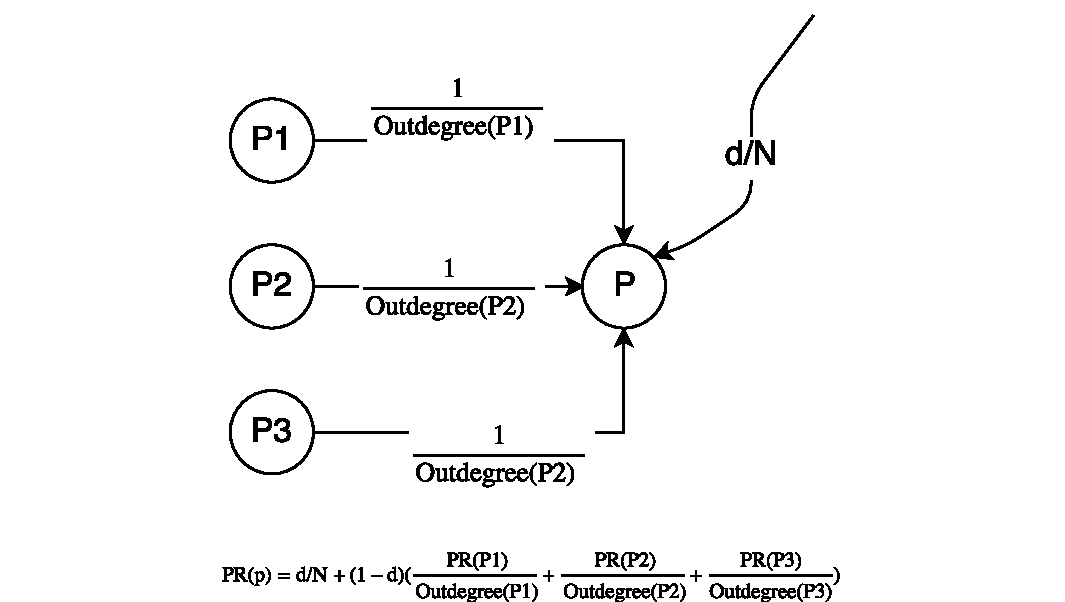
\includegraphics[max size={\textwidth}]{pagerank3.pdf}
  \caption{Příklad hodnocení stránky pomocí Markovova modelu náhodné stránky.}
  \label{pageRankFig}
\end{figure}

\subsection{Aplikace využívající datovou analýzu}
\par V průběhu využívání dolování dat a využívání datové analýzy se nástroje a aplikace postupně zdokonalovali a začínají být čím dál tím více uživatelsky přístupné. Firmy se snaží propojit několik takovýchto aplikací a dát uživatelům silné nástroje pro snadné a rychlé získání dodatečných informací z velkého množství dat. Často se objevuje možnost připojit různé zdroje dat do těchto aplikací.

\paragraph{Power BI} je sada obchodních analytických nástrojů od firmy Microsoft, tyto nástroje vynikají především možností připojení na velké množství datových zdrojů a také možností publikovat vytvořené reporty na webové rozhraní takzvaný dashboard. Pro připojení na různé datové zdroje je použit nástroj Power BI gateway, který umožňuje, mimo jiné, připojit na rázné SQL databáze a analytické modely. \cite{powerbi}

\paragraph{IBM Watson Analytics} hlavní motto tohoto nástroje je poskytnutí silných a pokročilých analytických technik bez přílišné komplexnosti. Výhodou oproti ostatním nástrojům a aplikacím je jednoznačně možnost rychle, a bez nutnosti pokročilých technik dolování dat, získat ukryté informace v zákaznických datech. Tohoto docíli inženýři ve firmě IBM tím, že vyvinuli velice silnou a rychlou umělou inteligenci, která má za úkol hledat skrytou podstatu v datech. \footnote{Více o této umělé inteligenci pojmenované Watson se můžete dočíst zde \url{http://www.slate.com/blogs/future_tense/2014/02/14/watson_is_real_artificial_intelligence_despite_claims_to_the_contrary.html}} \cite{watson}

\paragraph{MicroStrategy} platforma podporuje dashboardy, interaktivní reporty a dotazování, upozornění a mnoho dalšího potřebného pro vytváření strategie podniku a zjišťování informací z dat. Tato platforma nevyužívá klasické multidimenzionální OLAP kostky, ale využívá relační OLAP architekturu, což umožňuje možnost použítí nástroje drill down v jakékoliv dimenzi. Výhodou této platformy pro programátory je jistě dodávaný vývojářský balíček, který umožňuje dalšímu upravování vytvořených reportů a grafů. \cite{microstrategy}

\paragraph{SAP} nabízí hned dvě řešení pro možné dolování informací z dat \textbf{SAP BusinessObjects} a \textbf{SAP HANA}. První ze jmenovaných je sada fron-end aplikací která nabízejí uživateli prohlížet, řadit a pracovat s BI datami. Druhým je platforma, která má za úkol zpracovávat velké množství dat v reálném čase, jako bonus firma SAP nabízí vývojářský balík, kterým si uživatelé mohou upravit tuto platformu a rozšířit tak její využití. \cite{sap}

\section{Databázové aplikační platformy}
\par Mnoho firem v současné době nabízí různá řešení platforem, které zobrazují a umožňují práci s daty bez nutnosti instalace sofistikovaného programu u uživatele, ale za pomoci webového rozhraní. Tyto aplikace jsou převážně inspirovány úspěchem aplkace excel od firmy Microsoft, který v aktuální době používá více než 1,2 miliardy uživatelů \footnote{Podle oficiální zprávy od Microsoftu v roce 2016 \url{http://www.windowscentral.com/there-are-now-12-billion-office-users-60-million-office-365-commercial-customers}}. \par Firma Microsoft začala v nedávné době využívat možnost sdílet dokument mezi uživateli, kteří v reálném čase vidí změny prováděné na daném dokumentu. Podobnou funkci nabízí také firma Google, nicméně již nenabízí plnohodnou aplikaci, kterou by měl uživatel nainstalovanou na počítači a která by umožňovala uživateli pracovat pohodlněji s dokumenty (jak tomu je při použití aplikací od firmy Microsoft).

\paragraph{Fusioo} je webová aplikace, která nabízí jednoduchou integraci v rámci týmu pro správu důležitých informací. Je zde možné si nastavit dashboard, který nabízí metriky, grafy a upozorňení. Jeho velkou výhodou je možnost provázanosti do kalendáře, díky teré je možné jednoduše managovat tým a jeho aktivity.

\paragraph{Ragic} tato platforma nabízí uživatelům možnost snadného přechodu z klasických excelových tabulek do datbázového světa bez nutnosti jejich pochopení. Hlavním tahákem této platformy je určitě její chytré a intuitivní vyhledávání a při zadávání dat možnost zapnutí validace pro jednotlivé položky. Oproti konkurenci nabízejí neobvyklé reporty jako například TODO listy, náleky, kontingenční tabulky a mapy.

\paragraph{Quickbase} je aplikace zaměřené na pokročilé uživatele, nenabízí příliš jednoduchý způsob zadání dat, nicméně dovoluje upravovat data v připojené databázi za pomoci nástroje, který připomíná Access od firmy microsoft. Tato platforma se zaměřuje převážně na vývoj aplikací bez nutnosti psát kód, takovéto aplikace poté může zákazník dále nabízet ostatním uživatelům. Firma nabízí možnost definovat přístupová práva k jednotlivým dokumentům, skrze nastavení přístupových práv pro jednotlivé skupiny. Aplikace disponuje jedním velice zajímavým nástrojem ganttovým diagramem, který napomáhá k rozvržení práce v rámci týmu a naplánování vývoje.

\paragraph{Knack} velice jednoduchá, nicméně snadno použitelná aplikace, která dovoluje uživatelům definovat databázi a následně ji spravovat oline pomocí webového rozhraní. V rámci definování dat je možné nastavit jejich strukturu -- určit jednotlivé typy pro záznamy, propojení -- jednotlivé záznamy mohou být navzájem propojené a získat tak další informace a uživatel také může definovat vzorce a formule. Nad konkurencí tento nástroj vede převážně díky možnosti snadno importovat a exportovat data.

\paragraph{Nintex workflow} platforma nabízí automatizaci procesů v rámci firmy, což znamená že zákazník může propojit jednotlivé aplikace (které jsou kompatibilní s aplikací nintex) a systémy do určité posloupností úkolů, které dostanou zaměstnanci. Výhodou této platformy je především možnost propojení do velkého portfolia firemních aplikací, jako například NetSuite, Microsoft Dynamics a SAP, případně je možné vyvolat akci v podobě odeslání emailu, nebo SMS.

\section{Management vztahu se zákazníky (CRM)}
\par Je v podstatě termín používaný pro označení strategií a technologií použitých společnostmi pro monitorování a zjišťování stavu co uživatelé dělají s jejich produkty -- používají se jak k monitorování webových aplikací, tak volání, chatování, mailů a sociálních sítí. Mezi funkce CRM patří \textbf{automatizace marketingu}, \textbf{automatizace prodeje}, \textbf{automatizace kontaktního centra} a \textbf{geolokační technologie}. \cite{crm}

\begin{itemize}
  \item \textbf{Automatizace marketingu} napomáhá marketingovému oddělení některé repetetivní úkoly provádět automaticky. Jako například při zavedení nového produktu není nutné psát každému zákazníku speciální email, ale nechat CRM systém vygenerovat speciálně cílenou reklamu pro každého zákazníka.
  \item \textbf{Automatizace prodeje} elimunuje snahu prodat stejný produkt vícekrát různýmy zaměstnanci. Napomáhá ve sledování kdo a s jakou úspěšností se snaží daný produkt komu prodat.
  \item \textbf{Automatizace kontaktního centra} usnadňuje komunikaci se zákazníky, dovoluje například nahrát zprávu, která se ozve všem zákazníkům s určitým problémem nebo dotazem (pokud se například problém nebo dotaz opakují).
  \item \textbf{Geolokační technologie} některé CRM systémy dokonce disponují geolokační službu na základě které může podnik zjistit prodej určitého produktu napříč státy. \cite{crm}
\end{itemize}

\subsection{Monitorování webové aplikace}
\par V rámci zjišťování chování zákazníků na stránce může firma sáhnout po speciálním softwaru, který dovoluje jejich přesné monitorování. Díky tomuto monitorování může firma zjistit například v jakém kroku nákupu produktu zákazník odešel ze stránky a hlavně firma díky tomuto nástroji získá možnost přilákat nové zákazníky díky zjištění chování stávajícíh zákazníků. \cite{the-ux-book}

\paragraph{Google analytics} je poskytován zdarma od firmy Google, poskytuje statistické a základní nástroje analýzy používání webové stránky. Kromě toho, že je produkt zdarma má další výhody v podobě napojení na další nástroje od firmy Google, jako například \textbf{AdWords} \footnote{Placená služba, která dovoluje zákazníkům předplatit si reklamu na webových stránkách.}. Služba nabízí základní grafy a reporty spolu s možností zobrazit je na dashboardu. Těhcto druhů dashboardu může být několik druhů -- základní, SEO analýza, sociální média, geografie, mobilní analýza, příchozí/odchozí a technický (uživatel si saozřejmě může vytvořit vlastní dashboard).

\paragraph{KissMetrics} je placená alternatica ke Google analytics, cílí především na velké webové stránky a nabízí mnoho způsobů jak monitorovat zákazníky. Mezi přední výhodu patří možnost identifikace uživatele ještě před jeho přihlášením, kdy se ukládá jeho pohyb do anonymního účtu a pokud se tento uživatel v budoucnu identifikuje všechna anonymní data se automaticky spárují s tímto účtem. Tento nástroj také nabízí mnohem jednodušší možnost nastavení A/B testování \footnote{A/B testování je v podstatě vytvoření dvou různých variant jedné stránky a testování, která je více úspěšnější mezi uživateli (více stráveného času, koupě produktu, více kliknutí na stránce ...)}, kdy není potřeba vytvořit dvě různé URL pro jednu stránku. Dále tento nástroj nabízí velice jednoduché nastavení sledování chování uživatelů na jednotlivých stránkách, kdy je velice snadné nastavit například sledování času stráveného na stránce, dobu vyplňování formuláře, pohyb kurzoru po stránce atd.

\section{Shrnutí}
\par Aplikace zaměřující se na ukládání a práci s daty pomocí webového rozhraní se zaměřují převážně na větší podniky, případně nemají tolik intuitivní uživatelské rozhraní. Dále rozšiřitelnost dostupných aplikací není snadná a nastavení uživatelských práv je pouze v mizivém množství dostupných aplikací. Proto se dále zaměříme na vývoj samostatné aplikace, která spojí myšlenky z aktuálních aplikací a využije opensource nástroje, které umožní snadnější práci s uživateli.

%------------------------------------------------------------------------------------------------------------------------------------------
% Navrhy
%------------------------------------------------------------------------------------------------------------------------------------------
\chapter{VLASTNÍ NÁVRHY}
\par Nástroj, který je součástí této práce se zaměří z velké části na uživatelské rozhraní a do jisté míry využije technologie a nástroje, které jsou dostupné a usnadní tak vývoj a nasazení nového nástroje. Dále se budeme věnovat  životaschopnosti tohoto nástroje a způsobem jakým bude vytvořený nástroj nabízen veřejnosti. Firmy, pro které bude tato aplikace doporučována jsou malé, až střední podniky, které pracují s větším množstvím dat a potřebují nějakým způsobem najít skryté informace. Celá aplikace je vyvíjena v rámci open-source licence, proto je možné najít celý její kód (všech částí) na adrese \url{https://github.com/Lumeer}.

\section{Návrh aplikace}
\par Aplikace je postavena na základě aplikačního serveru WildFly, který pracuje s moduly napsanými v jazyce Java. Základní rozdělení aplikace je na \textbf{Engine} (veškerá serverová logika) a \textbf{UI} (webové uživatelské rozhraní). Engine je připojen na databázi MongoDb, což je NoSql databáze. Výhodou tohoto nastavení je vysoká pružnost v rámci zapsaných dat a není tedy nutné přesně definovat závislosti v rámci databáze (každý zákazník si může definovat jiné důležité atributy pro každý projekt).

\par Další výhodou oddělení uživatelského rozhraní a samostatného Enginu je možnost lépe řídit vývojářský tým, lépe rozdělit práci a v neposlední řadě, také možnost později vytvořit klienta nezávislého na dosavadním uživatelském rozhraní -- například vytvoření mobilní aplikace, která se bude specializovat na určitou část systému. Celý systém spolu komunikuje pomocí REST rozhraní a o zabezpečení se stará vrstva Keycloak, ve které jsou oba moduly registrovány a slouží jako takový středobod celého systému. Jak jsou jednotlivé části propojeny můžete vidět na obrázku \ref{schema}, kde hrany znamenají komunikační zprávy a uzly logické bloky.

\begin{figure}[!htp]
\centering
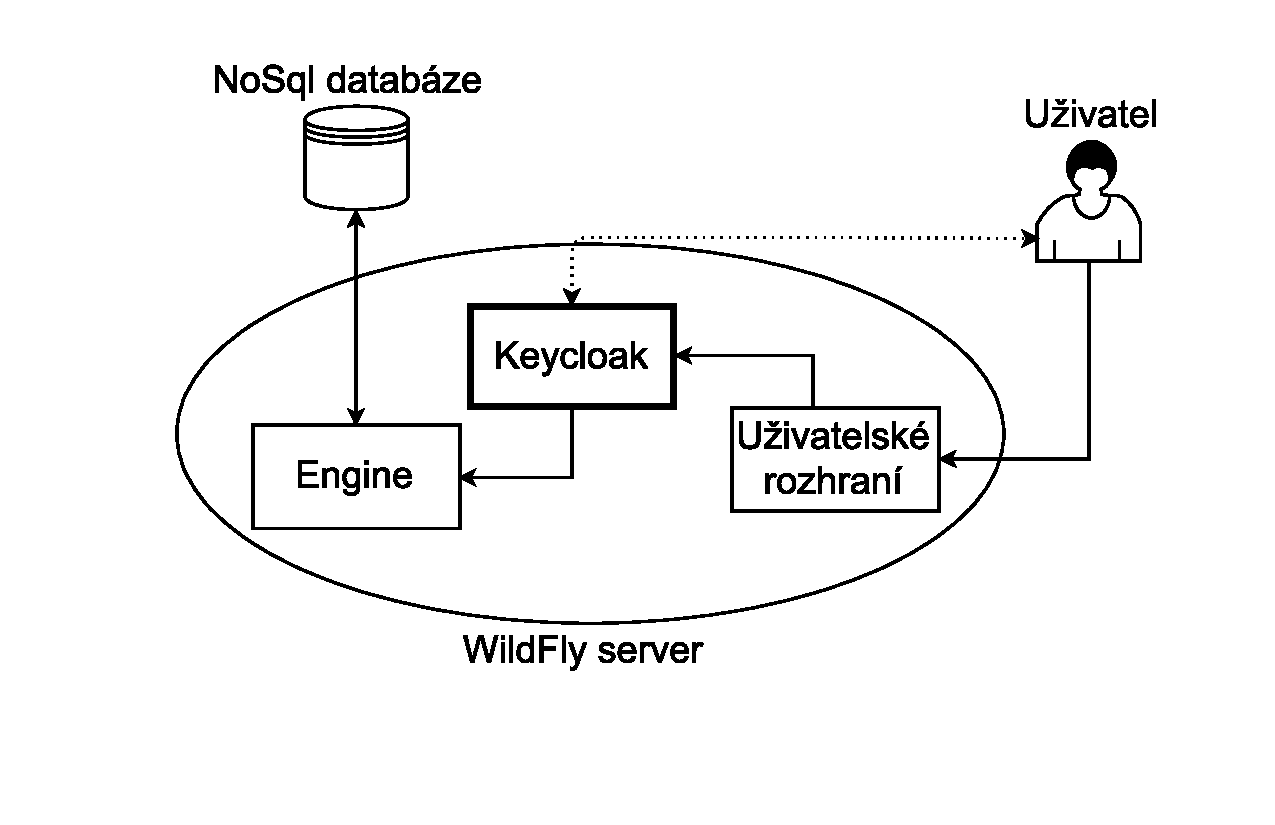
\includegraphics[max size={\textwidth}]{navrh.pdf}
\caption{Diagram znázorňující schéma nástroje.}
\label{schema}
\end{figure}

\par Pro znázornění jak dochází k získání dat se můžeme podívat na diagram \ref{komunikace}. Když uživatel vyvolá jakoukoliv akci, která vyžaduje získání dat ze serveru, uživatelské rozhraní se nejdříve zeptá Keycloak serveru, zda má aktivní token stále validní a pokud ne, autentizační server mu vytvoří nový. Poté uživatelské rozhraní pošle dotaz na samotný engine (v tomto dotazu se nachází autentizační token), kde se zkontroluje opět životnost tokenu, a zda má uživatel práva pro daná data. Pokud je vše v pořádku, server vrátí data, pokud ne, odpoví chybovou hláškou. Výhodou takové komunikace je, že nezáleží na implementaci uživatelského rozhraní, to může být napsáno jak pomocí webových technologií (Javascript), tak jako mobilní aplikace.

\begin{figure}[htp]
\centering
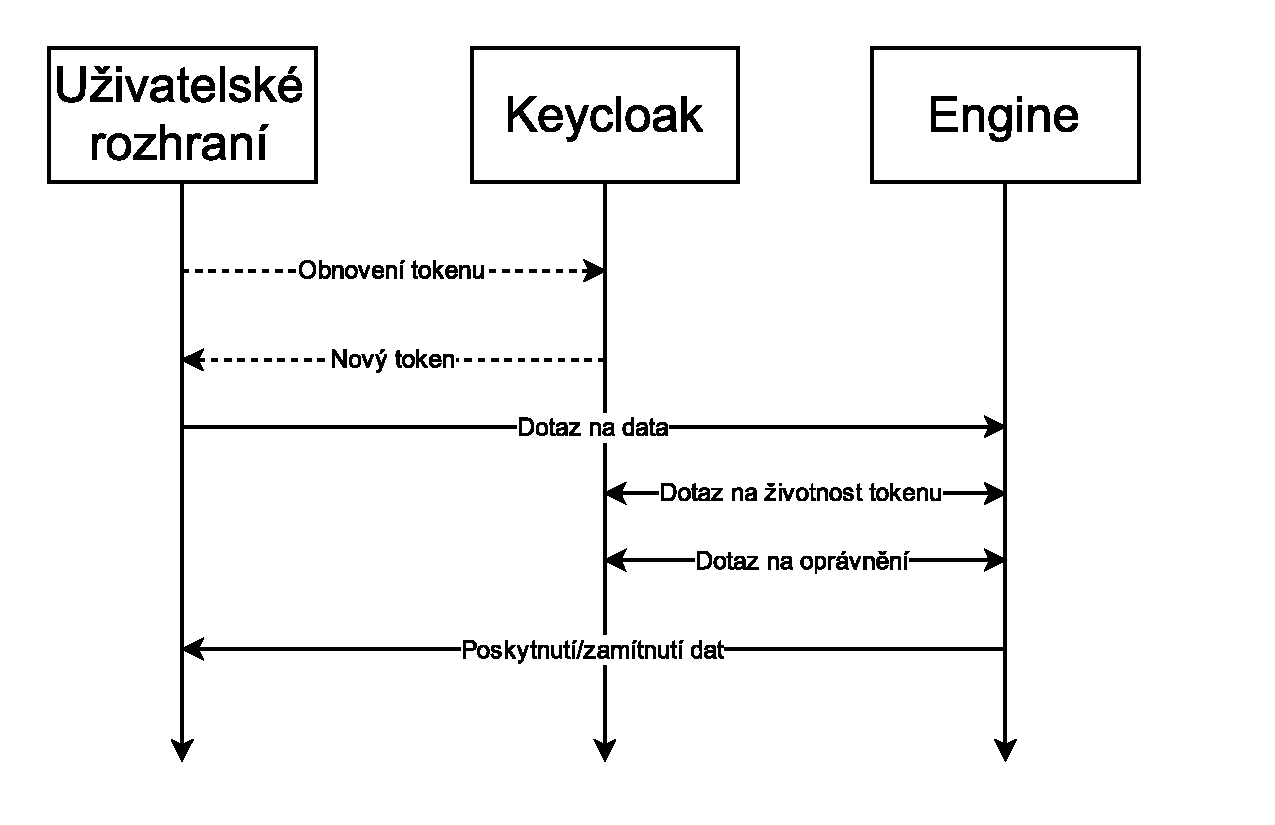
\includegraphics[max size={\textwidth}]{komunikace.pdf}
\caption{Diagram znázorňující schéma nástroje.}
\label{komunikace}
\end{figure}

\par Pokud uživatel již disponuje velkým datovým uložištěm je možné ho připojit do systému jednoduchou konfigurací v rámci UI. Systém prozkoumá tato data, některá si nakopíruje a začne je uživateli nabízet podobně, jako kdyby je uživatel měl již dříve v systému. Stejně je tomu s dolováním dat -- modul, který je zodpovědný za samostatné dolování, je možné připojit do systému, odkázat jej na datové uložiště a spustit dolování dat. Vše je nastavitelné jak z uživatelského prostředí, tak pomocí volání na předem definované RESTové služby.

\subsection{Vedení vývojového týmu}
\par Pro snadný a rychlý vývoj bylo nutné zvolit vhodné vedení vývojového týmu, který se podílel na vývoji celé aplikace. Ze zkušeností bylo určeno, že rychlého vývoje se dosáhne použitím agilní metody vedení týmu (inspirováno scrumem). Nicméně, protože jednotliví členové týmu se nenacházeli v dostatečné vzdálenosti, a nebyl tento projekt veden jako hlavní úkol jednotlivých členů, některá setkání, která jsou definována ve scrumu byla vyškrtnuta. Nejenom proto nelze vedení týmu, které bylo zvoleno, označit jako čistokrevný scrum, ale pouze jsme se při vedení inspirovali touto metodikou.

\par Nastavili jsme třítýdenní zveřejnění jednotlivých částí a každý týden jsme se scházeli, abychom si ujasnili na čem jaký člen týmu dělá a zda nemá nějaký problém. Použili jsme také nástroje určené ke snadnějšímu rozdělování práce, kdy jsme začali s používáním nástroje \textbf{Trello}\footnote{Jednoduchý nástroj, který vizualizuje aktuální práci za použití jednoduchých tabulí \url{https://trello.com/}.}, který nám postupně přestal stačit, a tak jsme využili opensource licence \textbf{Youtrack}\footnote{Tento nástroj je podobný Trellu, nicméně dovoluje snadnější a pro tým důležitou vizualizaci práce \url{https://www.jetbrains.com/youtrack/}.}

\subsection{Popis aplikační funkčnosti}
\par Před samotným popisem co a jak je propojeno, si musíme určit, co vlastně bude tato aplikace dělat a důvod jejího vzniku. Hlavním důvodem vzniku této aplikace je usnadnění editace často složitých záznamů (souborů) pomocí moderních technologií, záznamy můžeme rozumět například tabulky, grafy, kontingenční tabulky, atd. Mezi jednotlivými záznamy mohou vznikat a zanikat propojení, která umožní snadné napovídání datových záznamů a popisu dat (v případě tabulky si toto lze představit tak, že nám aplikace bude napovídat možné záhlaví tabulky a data v tabulce). Editování a nahlížení do záznamů bude povoleno pouze určitému uživateli. Dále jednotlivé soubory bude uživatel moci seskupovat do takzvaných kolekcí. Tímto dosáhneme jisté abstrakce nad soubory tak, aby uživatel přibližně tušil již při prvním pohledu na záznam, jaká data v něm mohou být. Vzhledem k tomu, že aplikace bude cílena na větší množství uživatelů, je možné aplikaci přepínat mezi různými projekty a organizacemi, takže uživatel může mít několik záznamů se stejným jménem ve stejné kolekci pod různými projekty a organizacemi.

\section{Použité technologie}
\par Může se zdát, že pro vytvoření tohoto nástroje bylo použito velké množství technologií, proto se následující kapitola bude věnovat jednotlivým částem aplikace -- jaké technologie přesně používá a jak jsou tyto technologie propojeny.

\subsection{Engine}
\par Základní část celé aplikace a její středobod se skládá ze tří pomyslných částí \textbf{Databáze}, \textbf{REST rozhraní} a \textbf{hlavní logika}. Díky tomuto rozdělení je možné snadno a hlavně rychle přidat novou funkcionalitu, dále je také možné rozdělit jednotlivé části vývojářům, kteří se mohou zaměřit na menší úkoly a pracovat tak efektivněji.

\par Hlavní logika byla naprogramována v jazyce Java a jako aplikační server poté použit Wildfly, díky jeho snadnému propojení do Keycloaku a také díky jeho robustnosti -- největší předností (aplikačního serveru wildfly) je jednoduché napojení na velké množství různých databází. K načtení závislostí, sestavení a nasazení tohoto modulu byl použit nástroj Maven.

\begin{itemize}
\item \textbf{Databáze} --  postavena nad technologií NoSql a přesněji použit databázový nástroj MongoDb. V pozdějším použití budeme pravděpodobně muset sáhnout po nějakém indexovacím nástroji  jako je například Elasticsearch nebo Solr, který nám umožní snadnější hledání napříč složitější databázovou strukturou.
\item \textbf{REST rozhraní} -- slouží pro snadnější přístup k jednotlivým datům a definuje jednoduše dostupné koncové uzly. Pokud bude potřeba nástroj rozšířit a hlavně zmapovat jednotlivé koncové uzly budeme moci použít například technologii Swagger\footnote{Slouží pro vizualizaci a zobrazení jaká data jednotlivý uzel očekává a jaké produkuje: \url{http://swagger.io/}.}
\end{itemize}

\subsection{Uživatelské rozhraní}
\par Hlavní část (Engine) funguje jako samostaný modul, který je nasazen do aplikačního serveru Wildfly, obdobně je tomu i v případě uživatelského rozhraní (samostatný modul, který je nasazena na Wildfly). Samotný proces sestavení používá nástroj \textbf{Webpack}, který celý zdrojový kód rozdělí do dvou Javascriptových souborů. Jeden obsahuje závislosti nutné pro chod aplikace a ve druhém je samostatný kód aplikace. V rámci usnadnění a jednoduššího přístupu k aplikaci jsme se rozhodli velkou část Javascriptových souborů umístit na veřejné CDN\footnote{CDN je v podstatě systém serverů, které nabízejí JS a CSS soubory uživatelům s ohledem na jejich geografickou lokaci, tak aby měli tyto soubory co nejdříve.}.

\par Vzhledem k rozsáhlosti a složitosti uživatelského rozhraní bylo rozhodnuto, že se použije aplikační framework s podporou jednostránkové aplikace. Po prozkoumání alternativ byl následně vybrán aplikační rámec \textbf{Angular 2}. S výběrem tohoto aplikačního rámce jde ruku v ruce také výběr jazyka ve kterém je uživatelské rozhraní napsáno, což je silně typovaný jazyk \textbf{Typescript}.

\par Uživatelské rozhraní se postupně upravovalo a byla snaha o co možná nejjednodušší používání této aplikace, proto byla první verze rozhraní představena několika méně zkušeným uživatelům počítače, kterým se dali jednoduché úkoly a byl sledován jejich postup a následně jim byla položena otázka, zda byl úkol snadný. Systém jim byl pouze zevrubně vysvětlen slovy, že se jedná o aplikaci, která obsahuje kolekce souborů, které jsou mezi sebou propojeny. Jak vypadalo uživatelské rozhraní před těmito úkoly se můžete podívat na obrázku \ref{old-ui}.

\begin{figure}[!h]
\centering
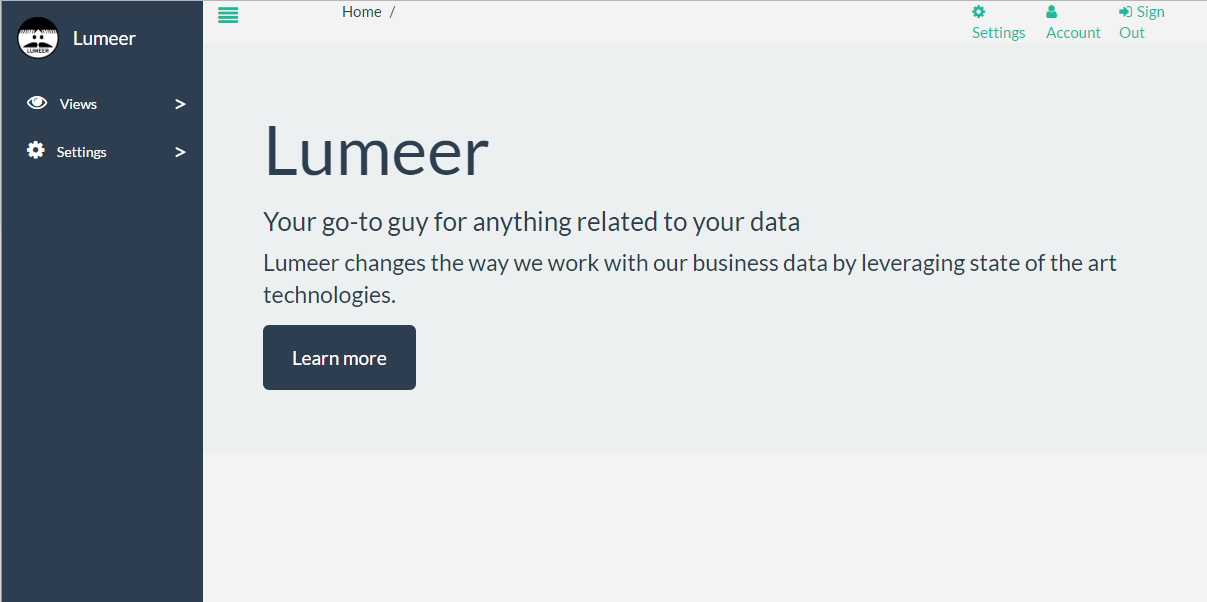
\includegraphics[max size={\textwidth}]{old-design}
\caption{Design aplikace před představením uživatelům.}
\label{old-ui}
\end{figure}

\subsubsection{Úkol číslo 1} Výběr kolekce a následné zjištění informací o této kolekci. Úrověň náročnosti: \textbf{lehká}. Na výsledky hodnocení lze vidět v tabulce \ref{ukol-1}.
\begin{table}[htp]
\begin{center}
\begin{tabular}{ || c || c | c | m{5cm} || }
\hline
Číslo uživatele & Rychlost vykonání & Ohodnocení & Slovní popis \\ [0.5ex]
\hline
\hline
1 & 25s & Snadný & Úkol se mi zdál ze začátku těžký, ale postupně jsem přišel na to kam kliknout. \\
\hline
2 & 38s & Středně těžký & Úkol se mi zádl celkem těžký a byl jsem docela zmatený s aplikací. \\
\hline
3 & 43s & Těžký & Vlbec jsem nechápal kam kliknout a potřeboval jsem pomoc. \\
\hline
\end{tabular}
\end{center}
\caption{Vyhodnocení úkolu číslo 1.}
\label{ukol-1}
\end{table}
\subsubsection{Úkol číslo 2} Výběr kolekce a dokumentu v kolekci pro který budou upraveny propojení. Náročnost: \textbf{středně těžká}. Výsledky hodnocení lze vidět v tabulce \ref{ukol-2}.
\begin{table}[htp]
\begin{center}
\begin{tabular}{ || c || c | c | m{5cm} || }
\hline
Číslo uživatele & Rychlost vykonání & Ohodnocení & Slovní popis \\ [0.5ex]
\hline
\hline
1 & 40s & Středně těžký & I po předhozím pochopení aplikace jsem měl s aplikací celkem problém.\\
\hline
2 & 48s & Těžký & Vůbec jsem něvěděl kam kliknout a co dělat. \\
\hline
3 & 1m 15s & Těžký & Potřeboval jsem hned od začátku pomoci a potřeboval jsem úkol několikrát vysvětlit a pomoci co dělat. \\
\hline
\end{tabular}
\end{center}
\caption{Vyhodnocení úkolu číslo 2.}
\label{ukol-2}
\end{table}
\subsubsection{Úkol číslo 3} Výběr kolekce a dokumentu v kolekci, pro který se zobrazí práva. Úroveň náročnosti: \textbf{těžká}. Výsledky hodnocení jsou k vidění v tabulce \ref{ukol-3}.
\begin{table}[htp]
\begin{center}
\begin{tabular}{ || c || c | c | m{5cm} || }
\hline
Číslo uživatele & Rychlost vykonání & Ohodnocení & Slovní popis \\ [0.5ex]
\hline
\hline
1 & 30s & Středně těžký & Vzhledem k tomu že tento úkol navazoval na předešlý, hned jsem věděl kde přibližně hledat. \\
\hline
2 & 52s & Těžký & Úkol navazoval na druhý a proto jsem přibližně věděl co a kam kliknout. \\
\hline
3 & 1m 10s & Těžký & Úkol byl podobný jako druhý úkol a proto jsem nepotřeboval takovou pomoc. \\
\hline
\end{tabular}
\end{center}
\caption{Vyhodnocení úkolu číslo 3.}
\label{ukol-3}
\end{table}

\par Vzhledem k výsledkům hodnocení a uživatelským podnětům se tým rozhodl přepracovat UI do více uživatelsky přívětivého způsobu. Hlavní výtkou všech uživatelů bylo příliš mnoho navigačních prvků na stránce, což vede k nepřehlednosti a uživatelé tak nevědí, na co kliknout a co použít. Na druhou stranu většina uživatelů, kterým byla aplikace představena zdůraznili výhodu vyhledávání a filtrování v rámci kolekcí, dokumentů a propojení. Z těchto poznatků bylo tedy určeno, že nejlepší bude zvýraznit vyhledávací formulář, který bude na všech stránkách aplikace. Dále také bude třeba sjednotit všechny prvky aplikace do jednoho vyhledávání tak, aby uživatelé měli přehledně a snadno dostupné například dokumenty a hned vedle nich propojení. Z těchto požadavků bylo tedy navrhnuto nové uživatelské rozhraní, které lze vidět na obrázku \ref{new-ui}.

\begin{figure}[htp]
\centering
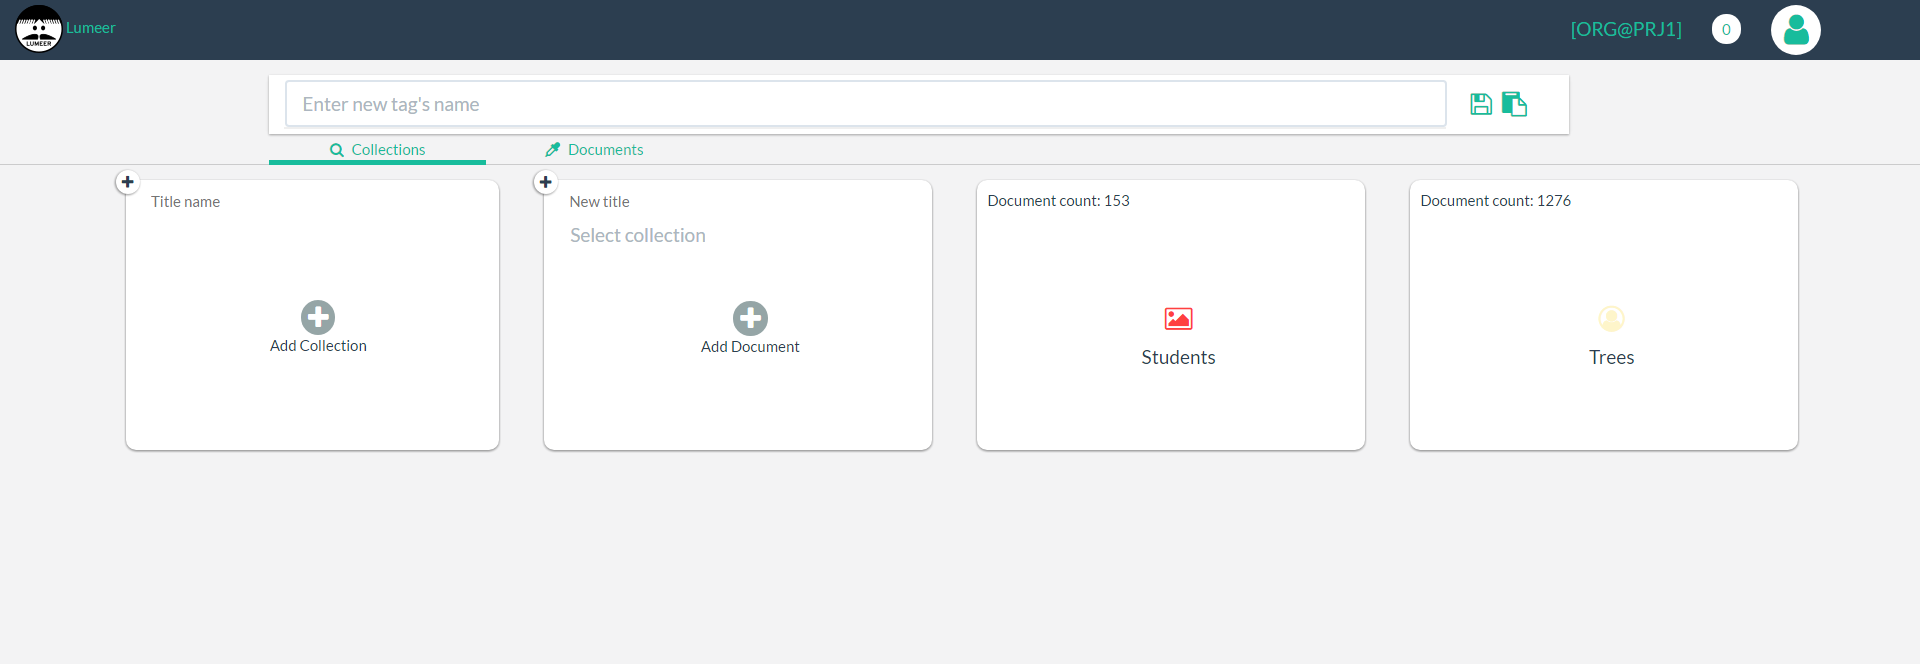
\includegraphics[max size={\textwidth}]{new-design}
\caption{Návrh nového uživatelského rozhraní.}
\label{new-ui}
\end{figure}

\subsection{Práce s grafy}
\par Díky tomu, že využíváme Webové technologie, můžeme jednoduše vytvořit grafy pro znázornění některých datových sad. Aplikace využívá více knihoven pro práci s daty, aby umožnila uživateli jednoduchou práci a možnost měnit typ grafů, upravovat datovou sadu, atd.

\subsubsection{Jednoduché grafy}
\par Pro znázornění a práci s jednoduchými grafy jsme využili knihovny \textbf{chart.js}. Tato knihovna se snadno ovládá a je jednoduchá pro nastavení; nicméně složitější grafické útvary nejsou jednoduché na vytvoření. Uživatel disponuje několika druhy grafů z této knihovny. Pokud chce používat komplexnější grafické znázornění musí si více připlatit a v aplikaci se zpřístupní možnost používat náročnější grafy, které jsou vytvořeny v knihovně \textbf{D3}. V základních operacích s grafy nabízí aplikace jednoduché sloupcové, spojnicové, koláčové a radarové grafy. Uživatel si může zvolit, z jakých datových sad bude čerpat data, jak je namapuje na grafy a případně možnost exportu grafu do pdf a obrázku.
\begin{figure}[!htb]
\centering
\subfloat[Sloupcový]{{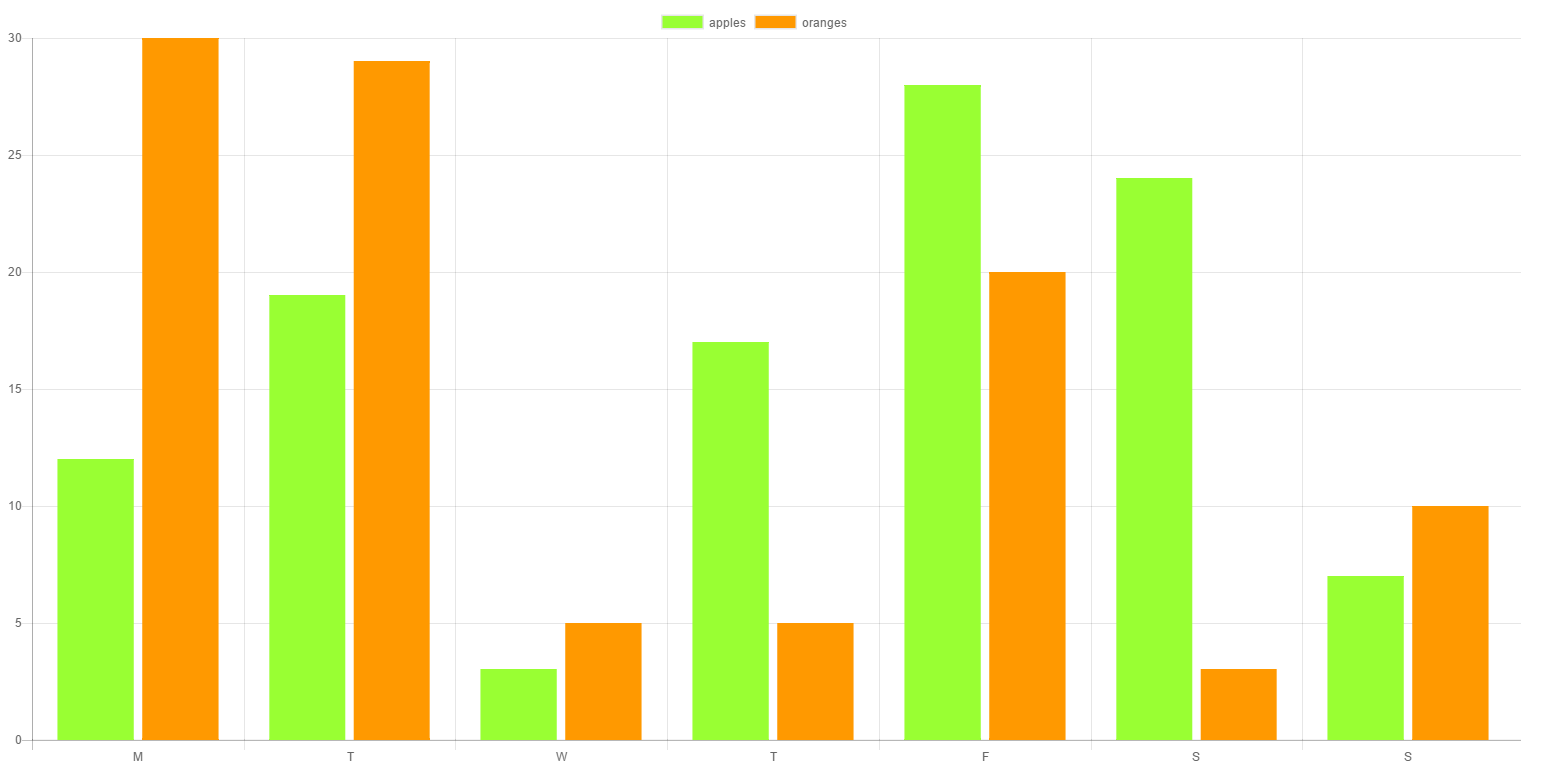
\includegraphics[width=5cm]{chart_bar} }}%
\subfloat[Spojnicový]{{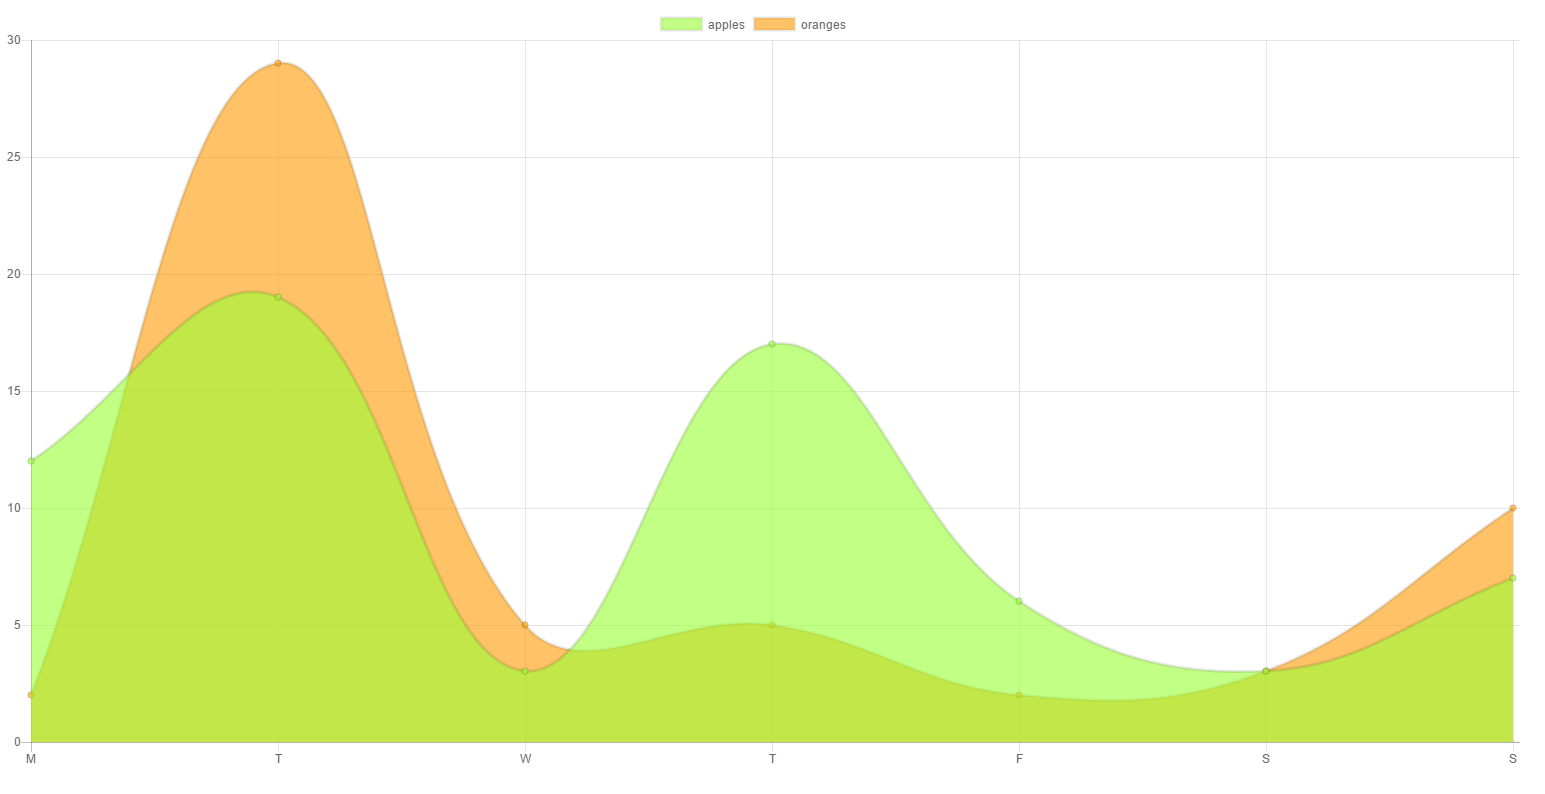
\includegraphics[width=5cm]{chart_line} }}%
\subfloat[Koláčový]{{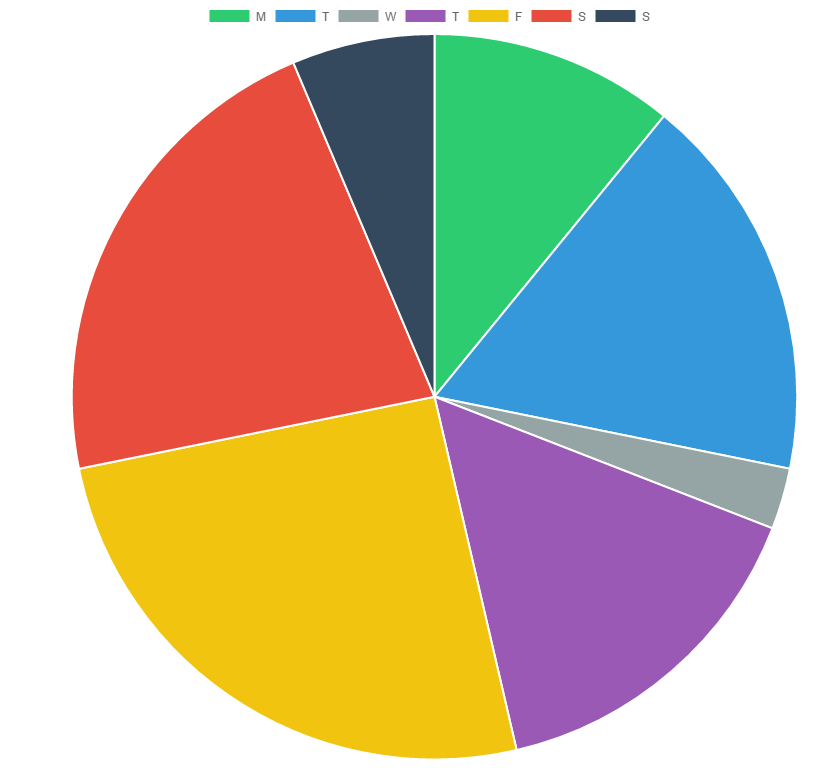
\includegraphics[width=5cm]{chart_pie} }}%
\caption{2 Figures side by side}%
\label{fig:example}%
\end{figure}

\subsubsection{Složitější grafy}
\par Jak již bylo nastíněno v předešlé sekci pro platící uživatele nabízí aplikace rozšířenou práci s grafy, převážně komplexnějších typů grafů se kterými může uživatel pracovat. Také možnost exportovat grafy do formátu, který přečte aplikace Microsoft Excel. Ale hlavní výhodou oproti jednoduchým grafům má použití knihovny D3 -- ta nabízí velké možnosti vytvoření jak grafů, tak různých grafických prvků. Tato knihovna je používaná nadstavbou \textbf{C3}, která definuje základní grafy, které je jednoduché vytvořit, ale je značně rozšiřitelná. Také v rámci složitější práce s grafy nabízíme uživateli možnost importovat data z různých formátů (CSV, XLS, XLSX atd.) a poté zvolit dokument, do kterého se tato data vloží, případně pouze pracovat s těmito daty a vytvořit graf, který poté může uživatel uložit jako samostatnou entitu.

\subsection{Vyhledávací jazyk}
\par Vzhledem k tomu, že součástí požadavků na aplikaci bylo také možnost jednoduše filtrovat a hledat v jednotlivých entitách, museli jsme přijít s vyhledávacím jazykem, který pokryje jak složité vyhledávací dotazy, tak je pro uživatele jednoduchý pro pochopení.

\subsubsection{Z pohledu uživatelského rozhraní}
\par Pomocí uživatelského rozhraní může uživatel zadat vyhledávací text dvojím způsobem -- \textbf{Fulltext}, nebo \textbf{tokeny}.

\par Pokud zvolí fulltextové vyhledávání, budou postupně uživateli napovídány jednotlivé texty napříč všemi entitami, tyto texty vytvoří nějakým způsobem větu, kterou odešleme na server a ten nám vrátí nejvhodnější výsledky. Součástí této funkcionality je také postupné překreslování vyfiltrovaných entit, které se objevují pod vyhledávacím polem.

\par V případě, že se uživatel rozhodne vyhledávat pomocí tokenů, usnadní serveru práci s odhadem co chce vyhledat a díky tomu dostane lépe sedící výsledky. Tokenizace probíhá tak, že si uživatel vybírá z předem definovaných prvků a z těch je postupně tvořen dotaz na server. Jak uživatel opět vytváří dotaz, jsou mu předávány prvky, které s velkou pravděpodobností hledá. Při použití tokenů uživatel získá také možnost hledat napříč několika entitami za použití logických operátorů, matematických operandů (větší, rovno, menší než) a textových (podobnost) operandů.

\par Pokud se tedy podíváme na tyto dvě metody, uživatel má možnost jednoduchého a rychlého hledání napříč aplikací pomocí fulltextového vyhledávání, nicméně toto vyhledávání není příliš vhodné pro složité dotazy. K tomu pak slouží tokenové vyhledávání, které je sice složitější, ale na druhou stranu přináší možnost hledat napříč velkým množstvím entit. Jako bonus si uživatel může tokenizované vyhledávání uložit jako filtr se jménem a následně v tokenizovaném filtru použít toto zástupné jméno. Může tedy postupně upravovat vnořené filtry, které může dále rozšiřovat a upravovat.

\subsubsection{Z pohledu serveru}
\par Pokud se zaměříme na vyhledávání z pohledu serveru musíme opět rozdělit tyto vyhledávací funkce na dvě části, stejně jako je tomu v případě uživatelského rozhraní.

\par Fulltextové vyhledávání je složitější pro server převážně kvůli tomu, že jako dotaz bude mít vždy jeden dlouhý řetězec, který musí rozpadnout do jednotlivých prvků a nad těmi provést výsledné vyhledávání v rámci databáze. Server funguje tak, že si větu nejdříve rozdělí do jednotlivých slov a ty roztřídí do binárního stromu -- jak lze například vidět na obrázku \ref{binarni-strom}, kde je věta \textit{Restaurant in Brno with burger and pizza}. Server zpracovává binární strom od spodu a vždy, když se mu povede vyhledat některý prvek, označí větev za vyřešenou a již ji dále nezpracovává. Takže při použití tohoto příkladu server zjistí, že uživatel hledá kolekci s názvem Restaurant, která obsahuje atribut Brno, dále server vyfiltruje všechny restaurace, které mají buger a které mají pizzu. Bohužel není vyhledávací algoritmus natolik přesný, aby vyhledal dokumenty ve kterých jsou tyto proměnné spojené.

\begin{figure}[!htb]
\centering
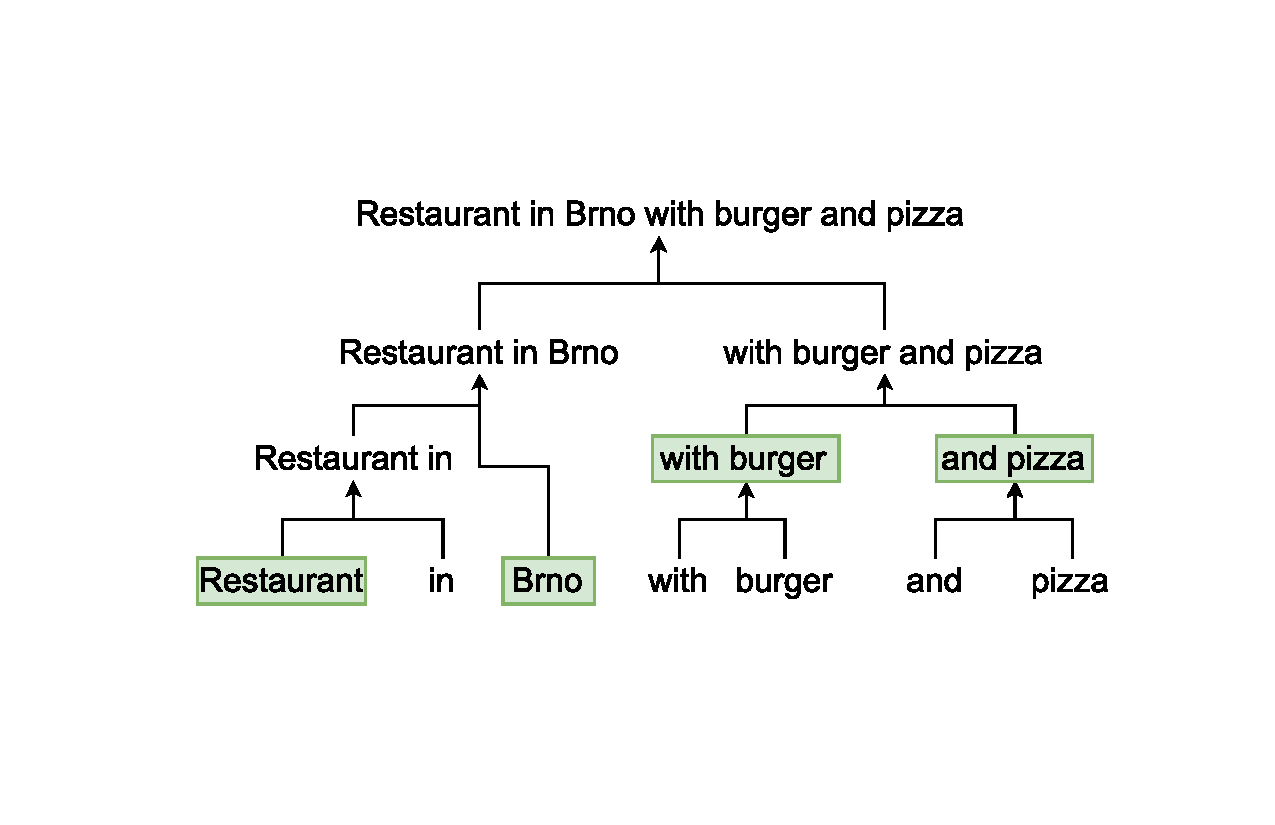
\includegraphics[max size={\textwidth}]{tree.pdf}
\caption{Binární strom pro roztřídění věty.}
\label{binarni-strom}
\end{figure}

\par Pokud uživatel použije tokenového, vyhledávání usnadní tak serveru následné hledání, protože nemusí složitě rozdělovat větu a skládat ji do strojově srozumitelného vyhledávání. Pokud například vezmeme opět větu \textit{Restaurant in Brno with burger and pizza}, tak ta by v tokenové verzi vypadala tak, že by vyhledávací dotaz obsahoval čtyři tokeny každý s informací o jednotlivých požadavcích. Tokenizované vyhledávání si uživatel může uložit do takzvaných pohledů, které může následně vyhledávat. Kliknutím na pohled se dostane rovnou na vyhledané entity skrz uložený dotaz.

\subsection{Zabezpečení}
\par V mnoha moderních aplikacích dochází k problémům se zabezpečením, ať již je to nedostatečné zabezpečení vůči případným útokům, nebo nechtěné dovolení přístupu různým uživatelům k datům, ke kterým by neměli mít přístup. Vytvářený nástroj se na toto téma snaží co nejvíce zacílit a použít řešení, které nebude příliš komplexní k nastavení pro zákazníka a zároveň bude poskytovat silné zabezpečení. Proto byl zvolen nástroj od firmy RedHat \textbf{Keycloak}, jehož fungování je popsáno v sekci o autentizačních serverech \ref{auth-server}.

\par V rámci tohoto nástroje je autentizační server nastaven tak, že před zapnutím aplikace je ověřeno přihlášení uživatele (díky nástroji Keycloak nemusí být uživatel přihlášen pouze k této aplikaci, ale k jakékoliv aplikaci spravované autentizačním serverem Keycloak, který má na starosti také tuto aplikaci). Pokud uživatel není přihlášen je vyzván k přihlášení, nástroj kromě klasického přihlášení pomocí emailu a hesla nabízí také možnost použít několik sociálních platforem -- Github, Facebook, Google účet a Twitter. Poté se již každý dotaz na server kontroluje tímto autentizačním serverem, takže je možné jednoduše nastavit pravidla uživatelům pro přístup jak k RESTovým službám, tak k jednotlivým zdrojům za pomoci Keycloak serveru a vytvořením skupin.

\par Díky autentizačnímu serveru se tedy v aplikaci nemusíme přímo starat o jednotlivé uživatele a nemusíme řešit zasílání hesel, celkovou správu a extra nastavení na serveru.

\section{Dolování dat}
\par Pokud vezmeme v úvahu hlavní modul starající se o dolování dat, můžeme ho rozdělit na tři části:
\begin{enumerate}
  \item \textbf{Heuristiky pro automatické linkování} -- pokud vznikne, nebo je upraven nějaký dokument je spuštěna řada automatických metod, které provedou případné automatické spojení.
  \item \textbf{Nejčastěji používané entity} -- na mnoha místech se aplikace snaží usnadnit práci uživateli tím, že mu nabídne ty, které jsou nejčastěji používané.
  \item \textbf{Přibližné napovídání} -- technika, která umožní napovídat uživateli možné výsledky při hledání bez nutnosti vyplnění celého jména.
\end{enumerate}

\subsection{Heuristiky pro automatické linkován}
\par Systém disponuje několika heuristikami, které se snaží vyhledávat skrytý význam v jednotlivých dokumentech a napomáhat tak uživateli při propojování dokumentů. Vezměme si například dva dokumenty -- jeden obsahuje jména, příjmení a telefonní čísla, nazvěme ho \textbf{uživatelský dokument}. Druhý bude například \textbf{studentský dokument}, ten bude obsahovat spojená jména a příjmení studentů spolu s jejich celkovým prospěchem. Po vytvoření studentského dokumentu nemusí mít uživatel tušení, že existuje uživatelský dokument a nevytvoří tak manuální propojení, nicméně systém si označí tyto dva dokumenty jako potencionální spojení a při zadávání dat do dokumentu studentů nám bude napovídat jména a příjmení z uživatelského dokumentu. Propojení těchto dokumentů tedy vznikne automaticky. Uživatel o tomto propojení nemusí být nijak informován, ale na stránce detailu studentského dokumentu uvidí informativní hlášku, která mu sdělí, že vzniklo nové propojení. Tento link může dále uživatel upravit, případně ho může odstranit a systém mu již nebude napovídat jména a příjmení.

\par Toto automatické propojení vzniká na základě dvou heuristických technik a následného vyhodnocení pomocí složení dvou sloupců z jedné tabulky do druhé. Tímto docílíme jednoduchosti a hlavně rychlosti zadávání nových záznamů. Velkou výhodou této techniky je, že sloupce, které jsou označeny jako propojené a získávané z různých tabulek, se automaticky obnovují, takže v případě změny jména v souboru uživatelů se tato změna automaticky projeví také ve studentském dokumentu (opět lze tuto funkci vypnout pro celý dokument, případně pro jednotlivé záznamy).

\par Nad takto nově vzniklými propojeními lze provádět samozřejmě stejné operace jako v případě klasických propojení -- tedy definovat propojovací řetězec a jednoduché funkce. Nicméně při vytvoření jednoduchých funkcí uživatel bohužel ztrácí automatické znovunačtení záznamů. Pokud chce načíst změny v takových záznamech, musí si vyžádat načtení hodnot, které jsou následně uloženy do souboru.

\par Příklady takových propojení můžeme vidět na obrázku \ref{linkovani}, kde první tabulka s názvem Nabízené zboží získává data ze dvou tabulek a poté další tabulka o (Věk a pohlaví uživatelů) čerpá jména z dokumentu, který obsahuje všechna možná jména.

\begin{figure}[htp]
\centering
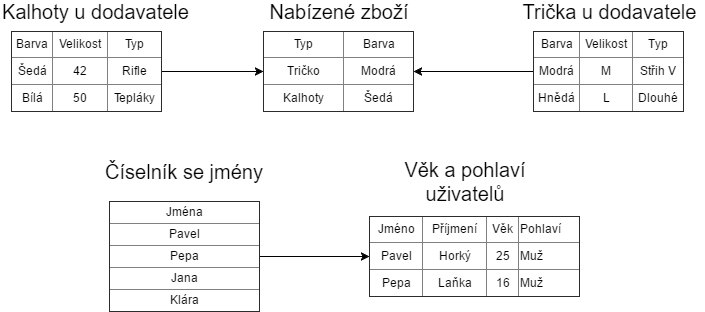
\includegraphics[max size={\textwidth}]{linkovani}
\caption{Příklad automaticky prolinkovaných dokumentů.}
\label{linkovani}
\end{figure}

\subsubsection{Heuristika 1}
\par V případě první heuristiky se kontrolují pouze záhlaví tabulky, takže pokud vezmeme v úvahu definovaný příklad, v momentě vytvoření dokumentu se provede kontrola nad podobnými soubory, a pokud se najde shoda, propojení se automaticky vytvoří.
\subsubsection{Heuristika 2}
\par Tato heuristika je složitější a znamená velkou zátěž pro systém, proto je potřeba dopředu provést nastavení tabulky při vytváření. Funguje tak, že při vytvoření nové tabulky uživatel může definovat tuto tabulku jako zdrojové data a kdykoliv se bude vytvářet nový soubor, provede se kontrola nad zdrojovými tabulkami, zda některá neobsahuje příslušný záznam. Vzhledem k náročnosti na systém jsme se rozhodli, že tuto vlastnost odstupňujeme pro jednotlivé druhy zákazníků.

\subsection{Nejčastěji používané entity}
\par S přihlédnutím k uživatelským požadavkům obsahuje systém možnost zobrazit entity, které jsou nejčastěji používané daným uživatelem pro jednu organizaci a projekt. Pro zobrazení požadovaných entit jsme nejdříve vybrali algoritmus \textbf{fronta}, ale tento model se nám neosvědčil, protože se často stávalo, že nejpoužívanější entity mizely z rychlého výberu a méně časté se nacházely v nabídce, proto jsme do systému naimplementovali možnost přepnutí na takzvanou \textbf{frontu s počítadlem} -- možnost pouze pro zákazníky s kvalitnější podporou. Přepnutí těchto technik se poté nachází v uživatelském nastavení, takže každý uživatel je schopen si toto řazení změnit.

\subsubsection{Fronta}
\par Fronta funguje na stylu omezeného počtu záznamů, které mohou být zobrazeny, a pokud je tento počet překročen, poslední záznam, který byl zaktivován, je odstraněn. Toto řešení je dostačující, nicméně může nastat to, že entita, která je často otevíraná, zmizí z tohoto seznamu kvůli otevření několika stejných entit. Chování v aplikaci lze vidět na obrázku \ref{zasobnik}, kdy fronta obsahuje entity označené 1, 2, 3, 4 a 5. Uživatel otevřel nově entitu s označením c a entity v zásobníku jsou tedy (od spodu fronty) c, 1, 2, 3 a 4.
\begin{figure}[htp]
\centering
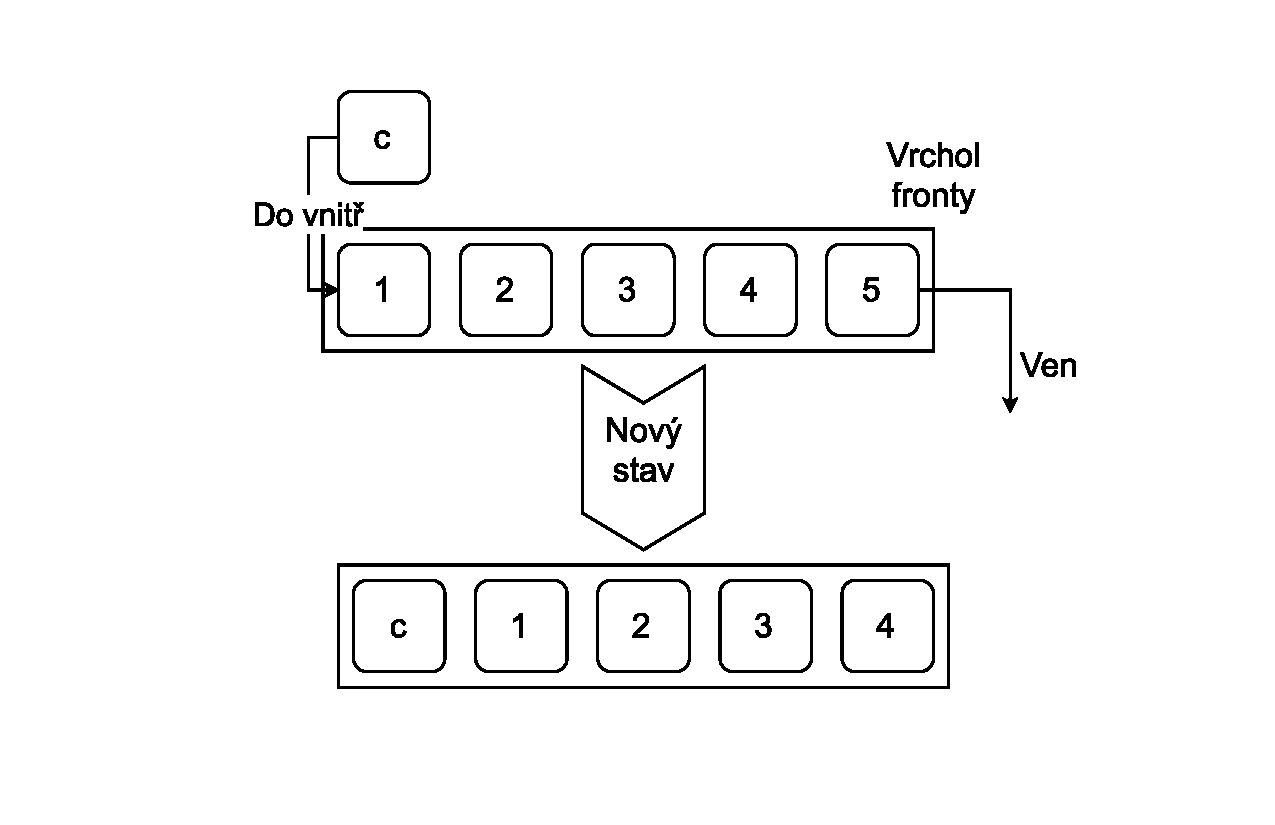
\includegraphics[max size={\textwidth}]{zasobnik.pdf}
\caption{Příklad plnění jednoduché fronty.}
\label{zasobnik}
\end{figure}

\subsubsection{Fronta s počítadlem}
\par Fronta s počítadlem je v podstatě rozšířená implementace fronty. Pokud je některá entita otevíraná častěji, je u ní zvyšován počet otevření. Entita s největším počtem otevření je na spodu fronty a entita s nejmenším počtem navrchu. Pokud se otevře nový dokument, je mu zvýšen počet otevření, a pokud překročí toto číslo nejvrchnější prvek ve frontě, tato nově otevřená entita nahradí tu, která byla na vrcholu fronty. Provedeno v rámci aplikace můžeme vidět na obrázku \ref{counter} -- nejčastěji používaná entita je označena 2 a nejméně používaná je označena 5; dále uživatel otevřel nově dokument s označením c a poté otevřel dokument d, který byl předtím otevřen jednou. Nově tedy zásobník obsahuje entity 2, 3, 4, 1 a d.
\begin{figure}[htp]
\centering
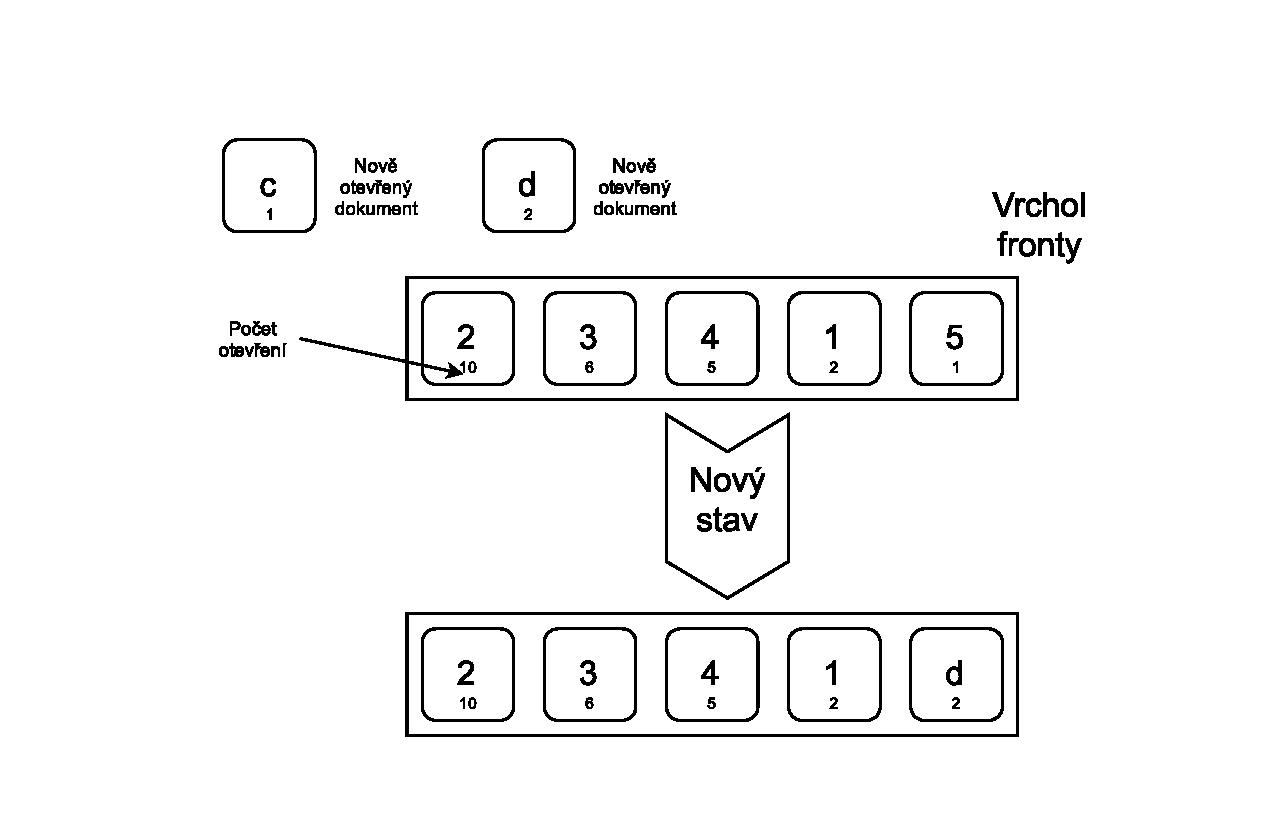
\includegraphics[max size={\textwidth}]{rozsireny-zasobnik.pdf}
\caption{Příklad plnění rozšířené fronty s počítadlem.}
\label{counter}
\end{figure}

\subsection{Přibližné napovídání}
\par Přibližné napovídání pracuje nad takzvanou fuzzy logikou a funguje na principu, že zadaný řetězec nemusí být vždy přesně zadán, aby uživateli byl dodán výsledek, který požaduje. Přibližné napovídání v aplikaci přibližné napovídání funguje tak, že v momentě, kdy uživatel zadá hledaný řetězec, jsou mu zobrazeny záznamy, které se nejblíže shodují k danému řetězci (případně obsahují prvních pár písmen), ideálně jsou tyto řetězce shodné. Aplikace nabízí možnost zobrazit uživateli entity, které mají v názvu nebo v možných řetězcích jedno písmeno jiné. Pokud uživatel následně vybere entitu, je k ní tento hledaný řetězec přidán. Entita tedy obsahuje seznam možných hledaných řetězců, které se dále mohou lišit o jedno písmeno. Například pokud budeme hledat entitu s názvem \textbf{Restaurace}, tato entita dále obsahuje seznam možných hledaných řetězců -- například \textit{Rez}, \textit{taue}, \textit{auea} a \textit{Res}. Uživatel tak zadá do hledání \textbf{Restaues} a systém mu nabídne entitu \textbf{Restaurace}.

\section{Analýza rizik}
\par Vzhledem k tomu, že vytvořit náročnou aplikaci není triviální, na začátku vývoje jsme si vytvořili analýzu možných rizik, na která můžeme narazit během vývoje a při distribuci. Také jsme si tato rizika ohodnotili a pro některé, které by měli vysoký dopad na aplikaci, jsme si připravili riziková opatření.

\par Následující tabulky znázorňují pravděpodobnost výskytu a dopad rizika.
\begin{table}[!htb]
    \begin{minipage}{.5\linewidth}
      \centering
\begin{tabular}{|c | c |}
\hline
Pravděpodobnost&Hodnota\\
\hline
0 - 20 \%&1\\
\hline
20 - 40 \%&2\\
\hline
40 - 60 \%&3\\
\hline
60 - 80 \%&4\\
\hline
80 - 100 \%&5\\
\hline
\end{tabular}
    \end{minipage}%
    \begin{minipage}{.5\linewidth}
      \centering

\begin{tabular}{|c | c |}
\hline
Hodnota&Dopad\\
\hline
1&Velmi nízký\\
\hline
2&Nízký\\
\hline
3&Střední\\
\hline
4&Vysoký\\
\hline
5&Velmi vysoký\\
\hline
\end{tabular}
    \end{minipage} 
    \caption{Ohodnocení pravděpodobnosti a dopadu rizika.}
\end{table}

\par Po vytvoření základních tabulek pro odhadnutí rizik jsme jednotlivá rizika zapsali do tabulky a ohodnotili jsme je možnou pravděpodobností a dopadem na funkčnost, nasazení nebo nepřijetí uživateli. jako mezní hodnotu jsme si určili 14 bodů při ohodnocení pravděpodobnosti a dopadu rizika -- výsledek je možné vidět v tabulce \ref{rizika}.

\begin{longtable}{ || c || m{3cm} | m{4cm} | c | c | c | c | }
\hline
Č. & Scénář & Hrozba & Pravděp. & Dopad & Hodnocení\footnote{Hodnocení = Pravděpodobnost * Dopad.}\\
\hline
\endhead
1 & Pomalý vývoj & S příchodem zákazníků budou přibývat požadavky na systém, které nemusíme stíhat přidávat & 2 & 3 & 6 \\
\hline
2 & Uživatelé nebudou rozumět aplikaci & Uživatelské rozhraní nebude intuitivní a snadno ovladatelné & 3 & 3 & 9 \\
\hline
3 & Nezabezpečená data & Kdokoli se dostane k uživatelským datům & 3 & 5 & \cellcolor{red!55}15 \\
\hline
4 & Napadení aplikace & Napadení aplikace třetí stranou & 2 & 5 & 10 \\
\hline
5 & Pomalá práce s daty & Při velkém objemu dat může nastat zamrzání aplikace & 4 & 3 & \cellcolor{yellow!55}12 \\
\hline
6 & Nezájem investorů & Aplikace nezujme případné investory, což povede k nedostatku zdrojů v prvotním spuštění & 3 & 5 & \cellcolor{red!55}15 \\
\hline
\caption{Možné scénáře rizik při vývoji a nasazení.}
\label{rizika}
\end{longtable}

\par Jak lze vidět v tabulce \ref{rizika}, tak pouze 2 rizika si vyžadují speciální pozornost, protože překračují námi definovanou hranici. Zaměříme se také na riziko s číslem \textbf{5}, které by mělo také kritický dopad na chod aplikace.

\begin{longtable}{ || c || m{3cm} | m{4cm} | c | c | c | c | }
\hline
Č. & Opatření & Cena & Pravděp.\_ & Dopad\_ & Hodnocení\_\footnote{Hodnocení = Pravděpodobnost\_ * Dopad.\_} \\
\hline
\endhead
3 & Při vývoji použijeme nástroj, který zabezpečí data & Cena nástroje pro zabezpečení & 2 & 5 & 10 \\
\hline
5 & Použití indexovacího nástroje & Cena nástroje pro indexaci dat & 3 & 3 & 9 \\
\hline
6 & Dedikování člověka pro komunikaci s investory & Cena člověka pro komunikaci & 2 & 5 & 10 \\
\hline
\caption{Opatření pro vyhnutí rizikům.}
\label{rizika}
\end{longtable}

\par Z možných opatření vyplývá že všem potencionálním technickým rizikům, ktera by měla vysoký dopad, se dá vyhnout použitím vhodných technologií a v případě rizika \textbf{6}, které by znamenalo možný nezájem investorů, musíme dedikovat člověka pro komunikaci a vytváření povědomí o tomto nástroji.

\par Pro znázornění zavedení opatření pro vyhnutí rizik jsme zvolili terčový graf \ref{risk-graph}, na kterém lze vidět, že žádné riziko nepřekračuje hodnotu 14 bodů, kteréou jsme si nastavili jako kritický bod. Nevěnovali jsme se rizikům, která nemají tak vysokou pravděpodobnost, že by nastala, nicméně i na ta je třeba dávat si pozor, a proto je dobré, že jsme na některá z nich narazili již na začátku.

\begin{graph}[ht]
\centering
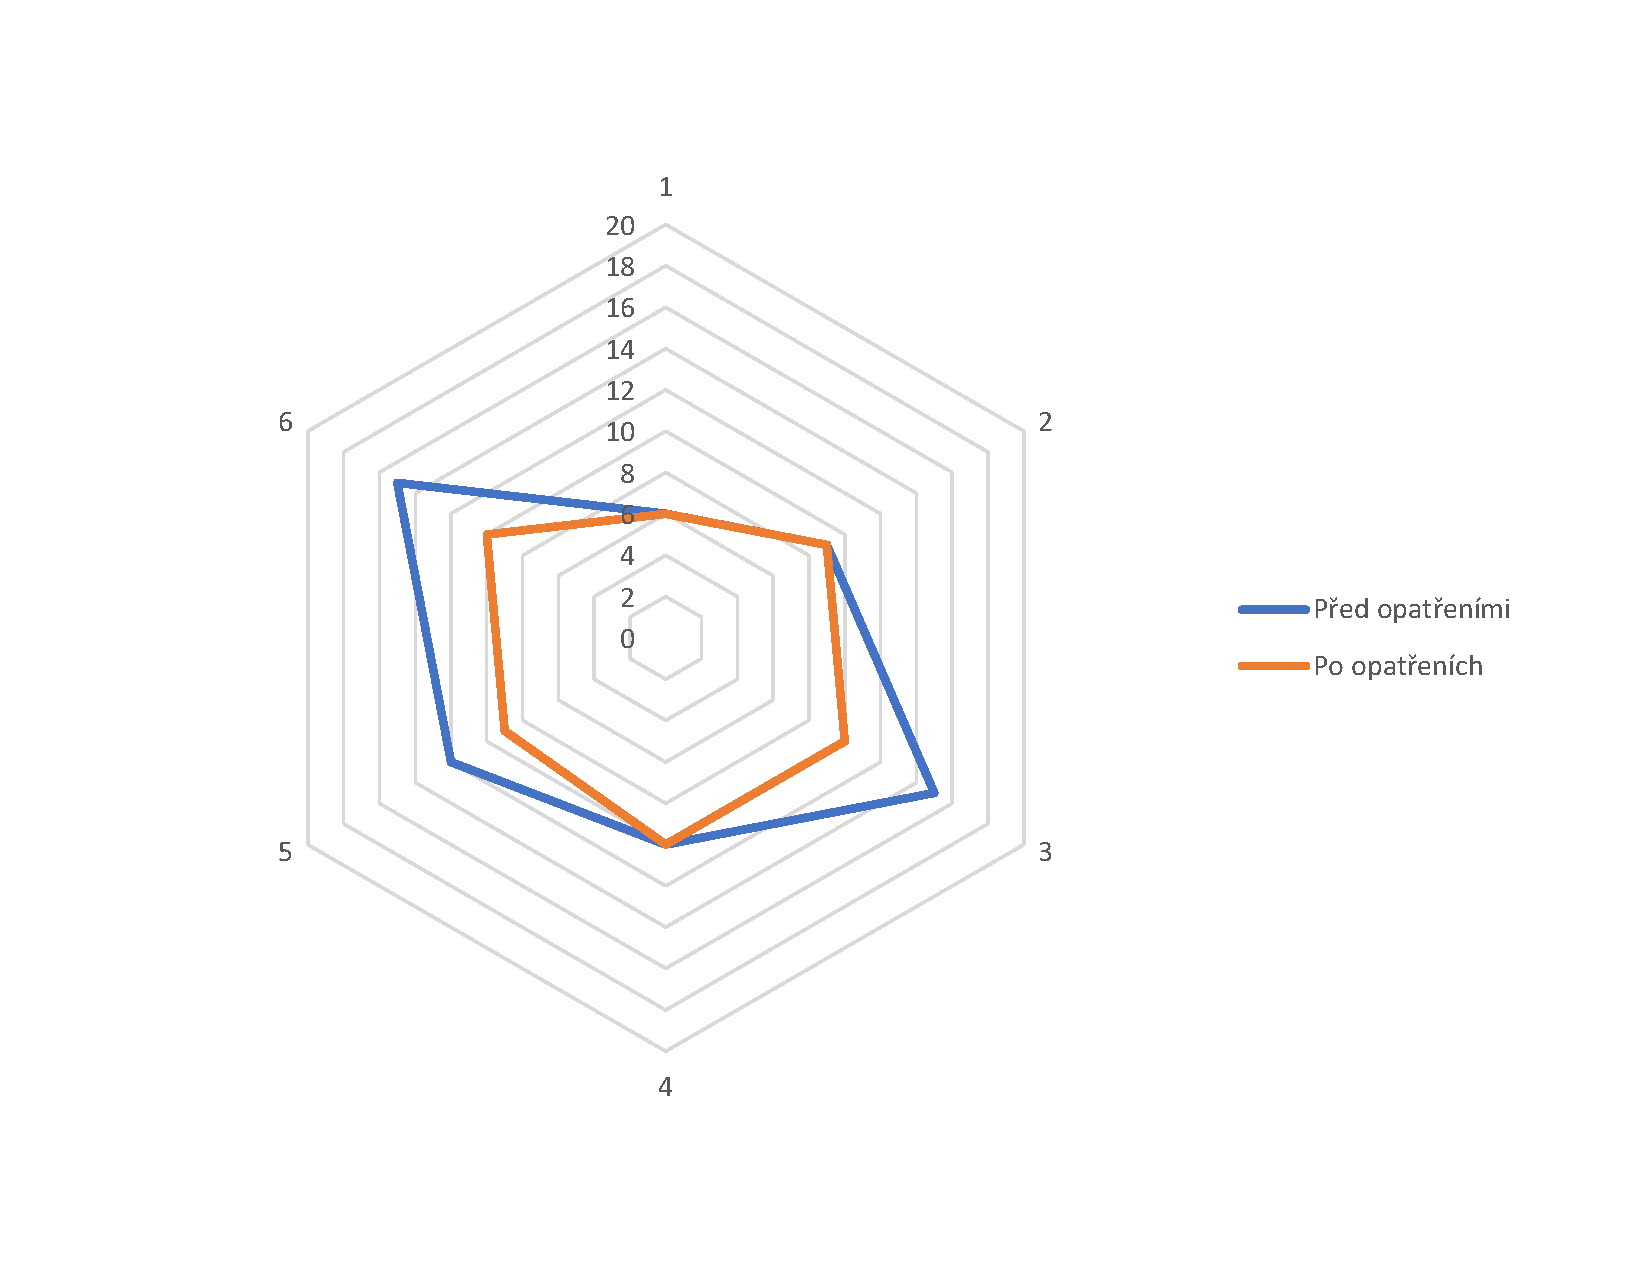
\includegraphics[max size={\textwidth}]{graph.pdf}
\caption{Rizika před a po zavedení rizikových opatření.}
\label{risk-graph}
\end{graph}

\section{Cenový model}
\par Jak již bylo několikrát řečeno v předchozím textu, aplikace se bude nabízet v několika cenových relacích, kdy více platící zákazníci dostanou na výběr větší množství funkcí a také větší podporu od vývojového týmu.

\par Cenový model můžeme shrnout do tří skupin -- \textbf{základní}, \textbf{střední} a \textbf{nejvyšší} (označováno též jako stříbrný, zlatý a platinový zákazník). Zákazníci si sami vyberou, jaké funkcionality se jim více hodí, přičemž první 2 měsíce mají zdarma na vyzkoušení. Takže zákazník dostane na začátku plnou podporu všech funkcí systému bez nutnosti platit jakoukoliv částku. V případě, že by chtěl školení, případně lepší podporu v těchto dvou měsících, je s ním vytvořena speciální smlouva, která může pokrývat tyto dva zkušební měsíce. Pokud nechce na začátku zákazník nic platit, nemusí, dostane návod jak aplikaci používat a menší ukázku toho, co s aplikací dělat a má možnost dva měsíce bezplatně testovat tento produkt.

\par Po uplynutí dvouměsíční lhůty si zákazník sjedná schůzku, kde se domluví bližší detaily přechodu do systému. Na začátku zákazník platí za služby jako například převod celé databáze, školení uživatelů, podporu při problémech a výpadcích atd. Každý úkon je ohodnocen individuálně na základě velikosti databáze (případně počtu uživatelů a jejich požadavků) a době strávené na přechodu pod systém.

\par Pokud zákazník souhlasí se všemi podmínkami a je ochotný začít používat aplikaci, je s ním také vytvořen speciální platící plán, ve kterém záleží na počtu uživatelů, kteří budou mít přístup k systému a k funkcionalitám, které jednotliví uživatelé požadují. Tento platící plán je opět individuální a nejvíce se mění v závislosti na počtu a druhu aktivovaných funkcí a na skupině zákazníka.

\par Vzhledem k tomu, že vývoj aplikace probíhá formou open-source, nemáme možnost, aby si schopnější uživatelé nevzali vyvýjenou aplikaci a nespustili si ji sami na svém vlastním stroji, tomuto se nijak nebráníme a je jasné, že takové případy budou vznikat, proto musíme sázet na to, že zákazníci budou chtít platit za podporu a za přidané hodnoty, na které mají nárok v rámci cenových modelů.

\chapter*{ZÁVĚR}
\par Cílem této práce bylo vytvořit platformu, která bude schopná pracovat s daty, vyhodnocovat jejich vnitřní informaci a následně nabízet uživateli jednoduché rozhraní pro práci s těmito daty.

\par Nejdříve bylo potřeba se seznámit s několika teoretickými pojmy, které byli důležité pro pochopení celého problému vývoje a návrhu takto rozsáhlé platformy. Vzhledem k tomu, že takováto platforma bude muset být často nasazena u několika zákazníků zároveň a že práce musí být plynulá a nemělo by záležet kde a jak ji uživatelé používají, proto bylo zvoleno použití webových technologií a k nim přidruženým nástrojům.

\par V rámci návrhu a vývoje platformy došlo k několika testování u různě schopných uživatelů, což mělo za následek částečnou změnu uživatelského rozhraní, a do podoby, která je snadná na používání a jednoduše pochopitelná.

\par Hlavní výhodou tohoto nástroje je jeho snaha o pochopení vnitřní informace v datech, které uživatel poskytne. Nad těmito daty se následně provádí několik funkcí, které nám pomohou s následným zpracováním tak, že uživateli jsou automaticky napovídány hodnoty, které již v systému jsou zapsány. Tímto se značně usnadňuje uživateli práce jak při zadávání nových hodnot, tak práce s již existujícími datovými sadami.

\par Během psaní této práce byl již nástroj představen několika případným investorům, kteří vyslovili velký zájem a chtěli by do něj přenést svá data. Někteří investoři sami chválí myšlenku této platformy a jsou spokojeni s jednoduchostí a snadným používáním.
\addcontentsline{toc}{chapter}{ZÁVĚR}
\newpage

\listoffigures
\addcontentsline{toc}{chapter}{Seznam obrázků}
\newpage
\listoftables
\addcontentsline{toc}{chapter}{Seznam tabulek}
\newpage
\addcontentsline{toc}{chapter}{Seznam rovnic}
\newpage
\listofequationcaps
\addcontentsline{toc}{chapter}{Seznam grafů}
\newpage
\listofgraphs
\addcontentsline{toc}{chapter}{Seznam zkratek}
\glsaddall
\printglossary[title=Seznam zkratek, nonumberlist]
\addcontentsline{toc}{chapter}{Seznam použitých zdrojů}
\begin{thebibliography}{99}

\bibitem{pcmag-no-coding}
MARVIN, Rob. Building an App With No Coding: Myth or Reality.
\textit{Pcmag}[online].
 Ziff Davis, LLC. PCMag Digital Group, 2016 [cit. 2017-03-11]. Dostupné z: \url{http://www.pcmag.com/article/345661/building-an-app-with-no-coding-myth-or-reality}
\bibitem{low-code-customer-want}
RUBENS, Paul. Use Low-Code Platforms to Develop the Apps Customers Want.
\textit{CIO} [online].
IDG Communications, 2014 [cit. 2017-03-11]. Dostupné z: \url{http://www.cio.com/article/2845378/development-tools/use-low-code-platforms-to-develop-the-apps-customers-want.html}
\bibitem{low-code-accelerate}
MARVIN, Rob. How low-code development seeks to accelerate software delivery.
\textit{SD Times} [online].
BZ Media LLC., 2014 [cit. 2017-03-11]. Dostupné z: \url{http://sdtimes.com/low-code-development-seeks-accelerate-software-delivery/}
\bibitem{zoho-review}
Zoho Creator REVIEW.
\textit{Finances Online} [online].
[cit. 2017-03-11]. Dostupné z: \url{https://reviews.financesonline.com/p/zoho-creator/}
\bibitem{what-is-low-code}
CIOT, Thierry. What is a Low-Code Platform?
\textit{Progress} [online].
2016 [cit. 2017-03-11]. Dostupné z: \url{https://www.progress.com/blogs/what-is-a-low-code-platform}
\bibitem{openshift-overview}
OpenShift Origin Overview.
\textit{OpenShift Origin} [online].
[cit. 2017-03-11]. Dostupné z: \url{https://docs.openshift.org/latest/architecture/index.html}
\bibitem{cloud-computing-dummies}
HURWITZ, Judith.
\textit{Cloud computing for dummies}.
Hoboken, NJ: Wiley Pub., c2010. ISBN 978-0470484708.
\bibitem{cloud-computing}
ROME, C. H.
\textit{The cloud computing Book: The ultimate guide to mastering cloud computing}.
Fifth edition. Bernemouth: Imagine Publishing, 2015.
\bibitem{essentials-cloud}
CHANDRASEKARAN, K.
\textit{Essentials of Cloud Computing}.
Maiami: CRC Press, 2014. ISBN 978-1482205435.
\bibitem{co-je-paas}
Co je PaaS?: Platforma jako služba.
\textit{Microsoft Azure} [online].
[cit. 2017-03-12]. Dostupné z: \url{https://azure.microsoft.com/cs-cz/overview/what-is-paas/}

\bibitem{data-science-business}
TODO data science business
\bibitem{predictive-analytics}
TODO predctive analytics
\bibitem{big-data-anayitics}
TODO big data analytics
\bibitem{big-data-dummies}
TODO big data for dummies
\bibitem{data-mining-principles}
BRAMER, Max.
\textit{Principles of data mining}.
3rd edition. 2016. ISBN 978-1-4471-7306-9.
\bibitem{data-mining-practical}
TODO data mining principles
\bibitem{advanced-data-vizualization-platforms}
TODO the forrester wave advanced data visualization adv platforms q3 2012
\bibitem{serverless-singlepage-apps}
TODO Serverless Single Page Apps
\bibitem{SPA}
TODO 1617290750Single
\bibitem{interactive-data-reily}
TODO interactive-data-reily
\bibitem{the-ux-book}
HARTSON, H. Rex. a Pardha S. PYLA.
\textit{The UX Book: process and guidelines for ensuring a quality user experience}.
Boston: Elsevier, c2012. ISBN 978-0123852410.
\bibitem{rest-cookbook}
ALLAMARAJU, Subrahmanyam.
\textit{RESTful Web services cookbook}.
Sebastopol,CA.: O'Reilly, c2010. ISBN 978-0596801687.
\bibitem{cloud-security}
TODO cloud security
\bibitem{scotch-jwt}
TODO \url{https://scotch.io/tutorials/the-anatomy-of-a-json-web-token}
\bibitem{rfc-jwt}
TODO RFC \url{https://tools.ietf.org/html/rfc7519}

\bibitem{big-data-action}
MARZ, Nathan a James WARREN.
\textit{Big data: principles and best practices of scalable real-time data systems}.
ISBN 978-1617290343.
\bibitem{data-mining}
HAN, Jiawei, Micheline KAMBER a Jian PEI
\textit{Data mining: concepts and techniques}.
3rd ed. Haryana, India ; Burlington, MA: Elsevier, 2012. ISBN 9789380931913.
\bibitem{nosql}
SADALAGE, Pramod J. a Martin FOWLER
\textit{NoSQL distilled: a brief guide to the emerging world of polyglot persistence}.
Upper Saddle River, NJ: Addison-Wesley, c2013. ISBN 978-0321826626.

\end{thebibliography}



\end{document}
